\documentclass[11pt, a4paper]{article}
\usepackage[utf8]{inputenc}
\usepackage{amsmath,setspace,geometry}
\usepackage{amsthm}
\usepackage{amsfonts}
\usepackage[shortlabels]{enumitem}
\usepackage{rotating}
\usepackage{pdflscape}
\usepackage{graphicx}
\usepackage{bbm}
\usepackage[dvipsnames]{xcolor}
\usepackage{hyperref}
\hypersetup{colorlinks=true, linkcolor= BrickRed, citecolor = BrickRed, filecolor = BrickRed, urlcolor = BrickRed, hypertexnames = true}
\usepackage[]{natbib} 
\bibpunct[:]{(}{)}{,}{a}{}{,}
\geometry{left = 1.0in,right = 1.0in,top = 1.0in,bottom = 1.0in}
\usepackage[english]{babel}
\usepackage{float}
\usepackage{caption}
\usepackage{subcaption}
\usepackage{tikz}
\usepackage{booktabs}
\usepackage{pdfpages}
\usepackage{threeparttable}
\usepackage{lscape}
\usepackage{bm}
\setstretch{1.4}
%\usepackage[tablesfirst,nolists]{endfloat}

\newtheorem{theorem}{Theorem}
\newtheorem{assumption}{Assumption}
\newtheorem{lemma}{Lemma}
\newtheorem{definition}{Definition}
\newtheorem{proposition}{Proposition}
\newtheorem{claim}{Claim}
\newtheorem{corollary}{Corollary}
\newtheorem{example}{Example}
\DeclareMathOperator{\rank}{rank}


\title{An MPEC Estimator for Conduct Parameter Estimation in Homogeneous Goods Markets: The Case of Log-linear Specification}
\author{Yuri Matsumura\thanks{Department of Economics, Rice University. Email: Yuri.Matsumura@rice.edu} \and Suguru Otani \thanks{Department of Economics, Rice University. Email: so19@rice.edu
\\Declarations of interest: none %this is for Economics Letters
}}

\begin{document}



\maketitle
\begin{abstract}
    We propose a constrained generalized method of moments estimator (GMM) for estimating conduct parameters in homogeneous goods markets. We formulate the estimation as a mathematical programming with equilibrium constraints (MPEC) problem incorporating theoretical conditions for the unique existence of equilibrium prices. 
    Monte Carlo simulations confirm that in a log-linear model, the MPEC estimator performs better than the nonlinear system two-stage least square estimator in estimating conduct parameters in large sample sizes. %81 words
\end{abstract}

\noindent\textbf{Keywords:} Conduct parameters, Homogenous Goods Market, Mathematical Programming with Equilibrium Constraints, Monte Carlo simulation
\vspace{0in}
\newline
\noindent\textbf{JEL Codes:} C5, C13, L1

\bigskip

\section{Introduction}
Measuring competitiveness is a crucial task in the empirical industrial organization literature.
Conduct parameter is considered a useful measure of competitiveness. 
However, it cannot be directly measured from data because data usually lack information about marginal cost.
Therefore, researchers aim to identify and estimate the conduct parameter.

As the simplest specification, \citet{bresnahan1982oligopoly} considers identification of conduct parameters for the linear model. \cite{matsumura2023resolving} resolves the conflict on some identification problems between \cite{bresnahan1982oligopoly} and \cite{perloff2012collinearity}. 
However, researchers often implement alternative specifications, such as the log-linear model\citep{okazaki2022excess,merel2009measuring}. 
Regarding the log-linear model, the identification strategy is provided by \citet{lau1982identifying}, but  
estimation problems arise when searching parameters using standard solvers because the equilibrium condition given by demand and supply curves involves log-transformation. 
This is an obstacle to choosing a better specification of the demand and supply functions.

To overcome the problem, we propose an estimator based on the mathematical program with equilibrium constraints (MPEC) approach advocated by \cite{su2012constrained}. 
MPEC is a constrained optimization problem whose constraint structure contains equilibrium constraints. 
We show that the MPEC estimator performs better in estimating conduct parameters than the standard approach such as nonlinear system two-stage-least-squares (N2SLS) in large sample sizes.\footnote{\cite{merel2009measuring} and \cite{okazaki2022excess} use N2SLS.}


\section{Model}
Consider data with $T$ markets with homogeneous products.
Assume there are $N$ firms in each market.
Let $t = 1,\ldots, T$ be the index of markets.
Then, we obtain the supply equation:
\begin{align}
     P_t = -\theta\frac{\partial P_t(Q_{t})}{\partial Q_{t}}Q_{t} + MC_t(Q_{t}),\label{eq:supply_equation}
\end{align}
where $Q_{t}$ is the aggregate quantity, $P_t(Q_{t})$ is the demand function, $MC_{t}(Q_{t})$ is the marginal cost function, and $\theta\in[0,1]$, which is the conduct parameter. 
The equation nests perfect competition $(\theta=0)$, Cournot competition $(\theta=1 / N)$, and perfect collusion $(\theta=$ $1)$ \citep{bresnahan1982oligopoly}.

Consider an econometric model.
Assume that the demand and the marginal cost functions are written as follows: 
\begin{align*}
    P_t = f(Q_{t}, X^{d}_{t}, \varepsilon^{d}_{t}, \alpha), %\label{eq:demand}
    \\
    MC_t = g(Q_{t}, X^{c}_{t}, \varepsilon^{c}_{t}, \gamma),%\label{eq:marginal_cost}
\end{align*}
where $X^{d}_{t}$ and $X^{c}_{t}$ are the vector of exogenous variables, $\varepsilon^{d}_{t}$ and $\varepsilon^{c}_{t}$ are the error terms, and $\alpha$ and $\gamma$ are the vector of parameters.
We also have the demand- and supply-side instruments, $Z^{d}_{t}$ and $Z^{c}_{t}$, and assume that the error terms satisfy the mean independence condition $E[\varepsilon^{d}_{t}\mid X^{d}_{t}, Z^{d}_{t}] = E[\varepsilon^{c}_{t} \mid X^{c}_{t}, Z^{c}_{t}] =0$. 

\subsection{Log-linear demand and log-linear marginal cost}
Consider a log-linear model, which is a typical specification.
The demand and marginal cost functions are specified as
\begin{align}
    \log P_{t} &= \alpha_0 - (\alpha_1 + \alpha_2 Z^{R}_{t}) \log Q_t + \alpha_3 \log Y_t + \varepsilon^{d}_{t},\label{eq:log_linear_demand}\\
    \log MC_t &= \gamma_0 + \gamma_1 \log Q_t +  \gamma_2 \log W_{t} + \gamma_3 \log R_t + \varepsilon^{c}_{t},\label{eq:log_linear_marginal_cost}
\end{align}
where $Y_{t}$ is an excluded demand shifter, $W_t$ and $R_t$ are excluded cost shifters, and $Z_t^R$ is Bresnahan's demand rotation instrument.
%Since $\partial P_t/\partial Q_t = - (\alpha_1 + \alpha_2 Z_{t}^R) (P_t/Q_t) $, 
Then, Equation \eqref{eq:supply_equation} is written as
\begin{align}
    P_t &= \theta (\alpha_1 + \alpha_2 Z^{R}_{t}) P_t + MC_t.\label{eq:log_linear_supply_equation_direct}
\end{align}

By taking logarithm of Equation \eqref{eq:log_linear_supply_equation_direct} and substituting Equation \eqref{eq:log_linear_marginal_cost}, we obtain
\begin{align}
    \log P_t = - \log(1 - \theta(\alpha_1 + \alpha_2 Z^{R}_{t})) + \gamma_0 + \gamma_1 \log Q_t +  \gamma_2 \log W_{t} + \gamma_3 \log R_t + \varepsilon^{c}_{t}. \label{eq:log_linear_supply_equation}
\end{align}

%An obstacle to estimate parameters is log-transformation in Equation \eqref{eq:log_linear_supply_equation}. First, the standard numerical algorithm faces invalid errors when evaluating the term, $\log (1 - \theta (\alpha_1 + \alpha_2 Z^{R}_{t}))$, whose inner candidate value, $(1 - \theta (\alpha_1 + \alpha_2 Z^{R}_{t}))$, is negative. The problem is inevitable because the true values of parameters are unknown. As in practical situations, researchers may want to use multiple rotation demand instruments or conduct parameters varied with time- or market- fixed effects.\footnote{See \cite{michel2018estimating} for the case of differentiated goods markets.} Then, the problem regarding the term becomes severer because the number of parameters within the log term increases. Second, if researchers may want to specify the demand function as $P_t=\alpha_0-\left(\alpha_1+\alpha_2 Z_t^R\right) Q_t+\alpha_3 Y_t+\varepsilon_t^d$, then the supply equation \eqref{eq:log_linear_supply_equation} is changed to $P_t=\theta \alpha_2 Z_t^R Q_t+\theta \alpha_1Q_t+\exp(\gamma_0+\gamma_1 \log Q_t+\gamma_2 \log W_t+\gamma_3 \log R_t+\varepsilon_t^c)$ which is nonlinear in cost parameters and conduct parameter $\theta$. 
%When constructing moment conditions, researchers face the above problem on log-transformation which limit researchers' alternative set of potential specifications.

An obstacle in the estimation is log-transformation in Equation \eqref{eq:log_linear_supply_equation}.
The standard numerical algorithm stops with invalid errors when the inside of the log function, $1 - \theta (\alpha_1 + \alpha_2 Z^{R}_{t})$, becomes negative during the search for an optimizer.
This problem is not specific to the above model and happens in other specifications, such as a model with linear demand and log-linear marginal cost.

In this model, the number of equilibrium prices varies. 
The conditions for the uniqueness in the following proposition are used in our estimation. 
\begin{proposition}\label{prop:equilibrium_existence}
    Assume that $\alpha_1 + \alpha_2 Z^{R}_{t}\ne 0$. Let $\Xi = \gamma_0 + \gamma_1\frac{\alpha_0 + \alpha_3 \log Y_t + \varepsilon^{d}_{t}}{\alpha_1 + \alpha_2 Z^{R}_{t}} +  \gamma_2 \log W_{t} + \gamma_3 \log R_t + \varepsilon^{c}_{t}$.
    The number of equilibrium prices $P_{t}^*>0$ is determined as follows:
    \begin{itemize}
        \item When $1 - \theta (\alpha_1 + \alpha_2 Z^{R}_{t}) \le 0$, there is no equilibrium price,
        \item When $1 - \theta (\alpha_1 + \alpha_2 Z^{R}_{t}) >0$, 
        \begin{itemize}
            \item If $-\gamma_1/(\alpha_1+\alpha_2 Z^R) \ne 1$, there is a unique equilibrium price,
            \item If $-\gamma_1/(\alpha_1+\alpha_2 Z^R) =1$, there are infinitely many equilibrium prices when $\exp(\Xi) = 1 - \theta (\alpha_1 + \alpha_2 Z^{R}_{t})$, but there is no equilibrium price otherwise.
        \end{itemize}
    \end{itemize}
\end{proposition}
See the online appendix \ref{sec:appendix_proof} for the proof.




% \subsection{Log-linear demand and log-quadratic marginal cost}
% Next, we consider more nonlinear specification.
% Assume that the cost function is a log-quadratic form specified as:
% \begin{align}
%     \log MC_t &= \gamma_0 + \gamma_1 \log Q_t + \tilde{\gamma}_1 (\log Q_t)^{2} +  \gamma_2 \log W_{t} + \gamma_3 \log R_t + \varepsilon^{c}_{t}.
% \end{align}
% Then, the log aggregate quantity $\log Q_t $ is a solution of: 
% \begin{align}
%     (\log Q_t)^{2} + \frac{\gamma_1}{\tilde{\gamma}_{1}}\log Q_{t} +\frac{C}{\tilde{\gamma}_{1}} &= 0,
% \end{align}
% where $C=\alpha_0 + \alpha_3 \log Y_t + \log (1 - \theta (\alpha_1 + \alpha_2 Z^{R}_{t})) - \gamma_0  -  \gamma_2 \log W_{t} - \gamma_3 \log R_t + \varepsilon^{d}_{t} - \varepsilon^{c}_{t}$.
% Note that although this specification does not have an analytical solution, we can find numerically find a single positive solution.
\section{MPEC estimator}
To estimate parameters in the demand and supply equations, we use GMM estimation.
Among GMM estimators, the N2SLS estimator directly uses Equation \eqref{eq:log_linear_demand} and \eqref{eq:log_linear_supply_equation}, which leads to the log-transformation problem.
See online appendix \ref{sec:setting} and \ref{sec:n2sls} for the construction of N2SLS based on Section 14.2 of \cite{wooldridge2010econometric}.
To avoid the obstacle, we propose an estimator utilizing the MPEC procedure \citep{su2012constrained,dube2012improving}.

Let $\xi = (\alpha_0,\alpha_1, \alpha_2, \alpha_3, \gamma_0,\gamma_1, \gamma_2, \gamma_3, \theta)$ be the vector of parameters.
To estimate the parameters, we convert the conditional moment conditions, $E[\varepsilon_t^d\mid Z_t^d] = E[\varepsilon_t^c\mid Z_t^c]=0$, into unconditional moment conditions, $E[\varepsilon_t^d Z_t^d] = E[\varepsilon_t^cZ_t^c]=0$.
Using the demand function \eqref{eq:log_linear_demand} and the marginal cost function \eqref{eq:log_linear_marginal_cost} directly, the sample analog of the moment conditions is given as
\begin{align*}
    g(\xi) = \left[\begin{array}{l}
    \frac{1}{T}\sum_{t=1}^T{\varepsilon}^{d}_{t}(\xi)Z_{t}^{d} \\
    \frac{1}{T}\sum_{t=1}^T{\varepsilon}^{c}_{t}(\xi)Z_{t}^{c}
    \end{array}\right],
\end{align*}
where
\begin{align}
    \varepsilon_t^d(\xi) & =  \log P_{t} - \alpha_0 + (\alpha_1 + \alpha_2 Z^{R}_{t}) \log Q_t - \alpha_3 \log Y_t, \label{eq:residual_demand_mpec}\\
    \varepsilon_t^c(\xi) & = \log MC_{t} - \gamma_0 - \gamma_1 \log Q_t -  \gamma_2 \log W_{t} - \gamma_3 \log R_t \label{eq:residual_supply_mpec}.
\end{align}

For some weighting matrix $W$, we define an MPEC estimator as $\xi^{*}$ solving the problem
\begin{align}
    &\min_{\xi, \{MC_t\}_{t=1}^T}\ g(\xi)^\top W g(\xi)\\
    \text{ s.t.}\quad & P_t = \theta (\alpha_1 + \alpha_2 Z^{R}_{t})P_t + MC_t,\quad t = 1,\ldots, T\\
    & 0 \le MC_t,\quad t = 1,\ldots, T\label{eq:positive_mc}.
\end{align}
Constraint \eqref{eq:positive_mc} is necessary because $\log MC_t$ becomes invalid when $MC_t$ is negative.

As the main difference from N2SLS, the MPEC estimator avoids the log-transformation problem by putting the first-order condition as an equality constraint and regarding $MC_t$ as a variable for the minimization problem.
While we focus on the log-linear specification, MPEC allows for more flexible specifications on the demand and marginal cost.
The programming cost of MPEC is lower than that of N2SLS because MPEC does not need analytical equilibrium expressions for constructing moment conditions.

We also impose the following constraints:
\begin{align}
    &0\le\theta \le 1,\label{eq:conduct_constraint}\\
    &\alpha_1 + \alpha_2 Z_{t}^{R} >0, \quad \gamma_1>0 ,\quad t = 1,\ldots, T\label{eq:slope_constraint}\\
    &1- \theta(\alpha_1 + \alpha_2 Z_{t}^{R}) >0,\quad t = 1,\ldots, T.\label{eq:equlibrium_existence}
\end{align}
Constraint \eqref{eq:conduct_constraint} is a standard assumption on the conduct parameter.
Constraints \eqref{eq:slope_constraint} and \eqref{eq:equlibrium_existence} relate to the uniqueness of equilibrium prices. 
Constraint \eqref{eq:slope_constraint} implies the downward-sloping demand and upward-sloping marginal cost.








\section{Simulation results}\label{sec:results}

We compare MPEC estimation with N2SLS estimation with Constraints \eqref{eq:conduct_constraint}, \eqref{eq:slope_constraint}, and \eqref{eq:equlibrium_existence}.
%Second, we examine the Two-Stage-Least-Square (2SLS) model in which Ipopt is implemented for minimizing its supply side moments and the simultaneous equation model in which Ipopt is implemented for minimizing both demand and supply side moments. 
%We refer to the former as separate estimation and the latter as simultaneous estimation.
%These two estimation procedures are considered to be a middle ground between MPEC and standard approaches because these do not use equilibrium constraints but state-of-the-art constrained optimization solvers.
Table \ref{tb:loglinear_loglinear_sigma_1_simultaneous_non_constraint_theta_constraint_bias_rmse} presents the results.
First, as the sample size increases, the root-mean-square error (RMSE) and bias decrease for all models. 
Second, we focus on estimating the conduct parameter because the results in the other parameters are comparable.
When the sample size is $T=1500$, MPEC estimation has a smaller bias (0.014) and RMSE (0.217) than those under N2SLS with the constraint (-0.148 and 0.333).
These differences arise only from whether we solve log-transformation as a constraint.
% \footnote{Specifically, for some datasets, N2SLS converges to the different points from true values of cost constant and conduct parameters by giving extremely low conduct parameter estimates by trying to avoid the log-transformation problem, whereas MPEC converges to the close points to the true values.}
Third, the percentage of convergence in MPEC estimation is larger than N2SLS. 
Therefore, MPEC is a better estimation approach than N2SLS in estimating the conduct parameter in large sample sizes.

See online appendix \ref{sec:n2sls} and \ref{sec:additional_experiments} for a comparison of the GMM objective values, additional experiments under different variances of errors, comparison to N2SLS without constraints, and the results of a linear model. 
Our findings are robust.

\begin{table}[!htbp]
  \begin{center}
      \caption{Performance comparison}
      \label{tb:loglinear_loglinear_sigma_1_simultaneous_non_constraint_theta_constraint_bias_rmse} 
      % \subfloat[Separate]{
\begin{tabular}[t]{llrrrrrrr}
\toprule
  & Bias & RMSE & Bias & RMSE & Bias & RMSE & Bias & RMSE\\
\midrule
$\alpha_{0}$ & -0.442 & 1.669 & -0.122 & 0.943 & -0.017 & 0.612 & 0.007 & 0.267\\
$\alpha_{1}$ & -0.246 & 0.949 & -0.071 & 0.529 & -0.013 & 0.348 & 0.005 & 0.151\\
$\alpha_{2}$ & 0.022 & 0.173 & 0.013 & 0.106 & 0.006 & 0.068 & -0.001 & 0.030\\
$\alpha_{3}$ & -0.109 & 0.544 & -0.030 & 0.297 & -0.007 & 0.205 & 0.003 & 0.090\\
$\gamma_{0}$ & -0.356 & 1.739 & -0.321 & 1.248 & -0.200 & 0.855 & -0.031 & 0.388\\
$\gamma_{1}$ & 0.088 & 0.516 & 0.060 & 0.350 & 0.039 & 0.236 & 0.006 & 0.096\\
$\gamma_{2}$ & 0.040 & 0.399 & 0.035 & 0.260 & 0.024 & 0.172 & 0.004 & 0.073\\
$\gamma_{3}$ & 0.042 & 0.391 & 0.035 & 0.262 & 0.021 & 0.179 & 0.003 & 0.077\\
$\theta$ & 0.125 & 0.409 & 0.120 & 0.363 & 0.068 & 0.285 & 0.000 & 0.163\\
Runs converged (\%) &  & 97.400 &  & 98.300 &  & 98.900 &  & 100.000\\
Sample size ($T$) &  & 50 &  & 100 &  & 200 &  & 1000\\
\bottomrule
\end{tabular}
}\\
    % \subfloat[N2SLS without the parameter constraints]{
\begin{tabular}[t]{lrrrrrrrr}
\toprule
  & Bias & RMSE & Bias & RMSE & Bias & RMSE & Bias & RMSE\\
\midrule
$\alpha_{0}$ & -1.922 & 8.603 & -0.068 & 5.116 & 0.037 & 2.035 & 0.000 & 1.556\\
$\alpha_{1}$ & -0.299 & 1.314 & -0.010 & 0.785 & 0.005 & 0.312 & 0.000 & 0.240\\
$\alpha_{2}$ & -0.013 & 0.104 & -0.002 & 0.063 & 0.001 & 0.024 & 0.000 & 0.019\\
$\alpha_{3}$ & -0.165 & 0.774 & -0.007 & 0.472 & -0.004 & 0.185 & -0.001 & 0.152\\
$\gamma_{0}$ & -1.767 & 14.394 & -1.001 & 6.530 & -0.208 & 1.993 & -0.156 & 1.566\\
$\gamma_{1}$ & 0.255 & 1.949 & 0.132 & 0.838 & 0.034 & 0.229 & 0.027 & 0.174\\
$\gamma_{2}$ & 0.125 & 1.097 & 0.053 & 0.475 & 0.017 & 0.150 & 0.019 & 0.119\\
$\gamma_{3}$ & 0.099 & 0.903 & 0.062 & 0.481 & 0.007 & 0.149 & 0.014 & 0.120\\
$\theta$ & -0.098 & 0.441 & -0.060 & 0.421 & -0.061 & 0.319 & -0.058 & 0.281\\
Runs converged (\%) &  & 98.100 &  & 98.700 &  & 100.000 &  & 100.000\\
Sample size ($T$) &  & 100 &  & 200 &  & 1000 &  & 1500\\
\bottomrule
\end{tabular}
}\\
    \subfloat[N2SLS with Constraints \eqref{eq:conduct_constraint}, \eqref{eq:slope_constraint}, and \eqref{eq:equlibrium_existence}]{
\begin{tabular}[t]{llrrrrrrr}
\toprule
  & Bias & RMSE & Bias & RMSE & Bias & RMSE & Bias & RMSE\\
\midrule
$\alpha_{0}$ & -0.905 & 6.954 & 0.120 & 5.001 & 0.072 & 2.042 & 0.052 & 1.563\\
$\alpha_{1}$ & -0.141 & 1.053 & 0.018 & 0.768 & 0.010 & 0.313 & 0.008 & 0.241\\
$\alpha_{2}$ & -0.006 & 0.101 & 0.000 & 0.062 & 0.001 & 0.024 & 0.001 & 0.019\\
$\alpha_{3}$ & -0.088 & 0.620 & 0.007 & 0.475 & -0.001 & 0.186 & 0.003 & 0.152\\
$\gamma_{0}$ & -1.748 & 14.206 & -0.938 & 6.428 & 0.015 & 1.995 & 0.163 & 1.570\\
$\gamma_{1}$ & 0.254 & 1.927 & 0.129 & 0.825 & 0.018 & 0.226 & 0.003 & 0.170\\
$\gamma_{2}$ & 0.117 & 1.083 & 0.049 & 0.467 & 0.008 & 0.148 & 0.007 & 0.116\\
$\gamma_{3}$ & 0.098 & 0.890 & 0.058 & 0.478 & -0.001 & 0.148 & 0.003 & 0.118\\
$\theta$ & -0.100 & 0.441 & -0.072 & 0.424 & -0.121 & 0.351 & -0.148 & 0.333\\
Runs converged (\%) &  & 99.600 &  & 99.900 &  & 100.000 &  & 100.000\\
Sample size ($T$) &  & 100 &  & 200 &  & 1000 &  & 1500\\
\bottomrule
\end{tabular}
}\\
    \subfloat[MPEC ]{
\begin{tabular}[t]{lrrrrrrrr}
\toprule
  & Bias & RMSE & Bias & RMSE & Bias & RMSE & Bias & RMSE\\
\midrule
$\alpha_{0}$ & -0.614 & 5.995 & -0.213 & 4.315 & 0.077 & 2.034 & 0.063 & 1.555\\
$\alpha_{1}$ & -0.085 & 0.902 & -0.024 & 0.663 & 0.011 & 0.312 & 0.010 & 0.240\\
$\alpha_{2}$ & -0.028 & 0.105 & -0.022 & 0.073 & 0.000 & 0.025 & 0.001 & 0.020\\
$\alpha_{3}$ & -0.070 & 0.549 & -0.019 & 0.431 & -0.001 & 0.185 & 0.004 & 0.152\\
$\gamma_{0}$ & -5.106 & 15.922 & -2.379 & 6.990 & -0.375 & 1.959 & -0.398 & 1.533\\
$\gamma_{1}$ & 0.386 & 2.047 & 0.141 & 0.839 & 0.045 & 0.229 & 0.044 & 0.175\\
$\gamma_{2}$ & 0.190 & 1.155 & 0.054 & 0.475 & 0.022 & 0.150 & 0.027 & 0.120\\
$\gamma_{3}$ & 0.163 & 1.006 & 0.065 & 0.482 & 0.013 & 0.149 & 0.023 & 0.121\\
$\theta$ & 0.186 & 0.442 & 0.158 & 0.422 & -0.007 & 0.275 & 0.014 & 0.217\\
Runs converged (\%) &  & 100.000 &  & 100.000 &  & 100.000 &  & 100.000\\
Sample size ($T$) &  & 100 &  & 200 &  & 1000 &  & 1500\\
\bottomrule
\end{tabular}
}\\
  \end{center}
  \footnotesize
  Note: The error terms are drawn from a normal distribution, $N(0, \sigma)$. True values: $\alpha_0=20.0,\alpha_1=1.0,\alpha_2=0.1,\alpha_3=1.0,\gamma_0=5.0,\gamma_1=1.0,\gamma_2=1.0,\gamma_3=1.0,\theta=0.5$ and $\sigma=1.0$. See online appendix \ref{sec:setting} for the setting.
\end{table} 



\section{Conclusion}
We propose an MPEC estimator for conduct parameter estimation in homogeneous goods markets.
Our approach avoids the complex transformation within the equilibrium conditions and allows a broader set of specifications. 
Monte Carlo simulations confirm that the MPEC estimator performs better than N2SLS for estimating conduct parameters in a log-linear model in large sample sizes. 
%We conclude that MPEC enables us to estimate a broader set of specifications which are identified theoretically shown in \cite{lau1982identifying} but practically and numerically difficult to estimate.
% We revisit the conduct parameter estimation in homogeneous goods markets.
% There is a conflict between \citet{bresnahan1982oligopoly} and \citet{perloff2012collinearity} in terms of identification and estimation.
% We highlight the problems in the proof and simulation in \citet{perloff2012collinearity}.
% Our simulation shows that the estimation of the conduct parameter becomes accurate by appropriately introducing demand shifters into the supply estimation and increasing the sample size. 
% Based on the theoretical and numerical investigation, we support the argument in \citet{bresnahan1982oligopoly}.


\paragraph{Acknowledgments}
We thank Jeremy Fox, Yelda Gungor, and Isabelle Perrigne for valuable comments. This research did not receive any specific grant from funding agencies in the public, commercial, or not-for-profit sectors. 

\newpage
\bibliographystyle{aer}
\bibliography{conduct_parameter}

\newpage
\appendix

\section{Online appendix}
\subsection{Existence and uniqueness of equilibrium prices}\label{sec:appendix_proof}

Proposition \ref{prop:equilibrium_existence} proposes the conditions for the unique existence of $P_{t}(>0)$ solving the demand equation \eqref{eq:log_linear_demand} and supply equation \eqref{eq:log_linear_supply_equation} for $P_{t}$ under $\theta\in[0,1]$.
The proof is not based on the optimization by individual firms but checks if there exists a point at which the demand function and the marginal cost function cross.
Therefore, we allow an equilibrium price to exist when the demand and the marginal cost are upward-sloping.
    
\begin{proof}
    
% \begin{align}
%     \log P_{t} &= \alpha_0 - (\alpha_1 + \alpha_2 Z^{R}_{t}) \log Q_t + \alpha_3 \log Y_t + \varepsilon^{d}_{t},\\
%     P_t &= \theta (\alpha_1 + \alpha_2 Z^{R}_{t}) P_t + MC_t\nonumber\\
%     &=\theta (\alpha_1 + \alpha_2 Z^{R}_{t}) P_t + \exp(\gamma_0 + \gamma_1 \log Q_t +  \gamma_2 \log W_{t} + \gamma_3 \log R_t + \varepsilon^{c}_{t}).
% \end{align}
Rewriting the demand equation \eqref{eq:log_linear_demand} as 
\begin{align*}
    \log Q_{t}(P_{t})= \frac{\alpha_0 - \log P_{t} + \alpha_3 \log Y_t + \varepsilon^{d}_{t}}{(\alpha_1 + \alpha_2 Z^{R}_{t})}   
\end{align*}
and substituting this into the supply equation \eqref{eq:log_linear_supply_equation}, we obtain
\begin{align}
    P_t &=\theta (\alpha_1 + \alpha_2 Z^{R}_{t}) P_t + \exp\left(\gamma_0 + \gamma_1 \log Q_t(P_{t}) +  \gamma_2 \log W_{t} + \gamma_3 \log R_t + \varepsilon^{c}_{t}\right). \nonumber\\
    & = \theta(\alpha_1 + \alpha_2 Z^{R}_{t})P_t + \exp\left(\gamma_0 + \gamma_1 \frac{\alpha_0 - \log P_{t} + \alpha_3 \log Y_t + \varepsilon^{d}_{t}}{(\alpha_1 + \alpha_2 Z^{R}_{t})} +\gamma_2 \log W_{t} + \gamma_3 \log R_{t} + \varepsilon^{c}_{t} \right)\nonumber\\
    & = \theta(\alpha_1 + \alpha_2 Z^{R}_{t})P_t  + \exp\left(\Xi + \frac{-\gamma_1}{\alpha_1+\alpha_2 Z^{R}_t} \log P_t \right)\nonumber\\
    &= \theta(\alpha_1 + \alpha_2 Z^{R}_{t})P_t  + \exp(\Xi) P_t^{\frac{-\gamma_1}{\alpha_1 + \alpha_2 Z^{R}_{t}}} \label{eq:equilibrium_equation}
\end{align}
where $\Xi = \gamma_0 + \gamma_1\frac{\alpha_0 + \alpha_3 \log Y_t + \varepsilon^{d}_{t}}{\alpha_1 + \alpha_2 Z^{R}_{t}} +  \gamma_2 \log W_{t} + \gamma_3 \log R_t + \varepsilon^{c}_{t}$.

Any price that satisfies \eqref{eq:equilibrium_equation} becomes an equilibrium price.
To find an equilibrium price $P_{t}^*$, we define $\Delta(P_t)$ as follows:
\begin{align}
    \Delta(P_t)
    %&=P_t -\left(\theta (\alpha_1 + \alpha_2 Z^{R}_{t}) P_t + \exp(\gamma_0 + \gamma_1 \log (\frac{\alpha_0 - \log P_{t} + \alpha_3 \log Y_t + \varepsilon^{d}_{t}}{(\alpha_1 + \alpha_2 Z^{R}_{t})}) +  \gamma_2 \log W_{t} + \gamma_3 \log R_t + \varepsilon^{c}_{t})\right)\\
    &= \underbrace{[1 - \theta (\alpha_1 + \alpha_2 Z^{R}_{t})]P_t}_{(I)} - \underbrace{\exp(\Xi) P_t^{\frac{-\gamma_1}{\alpha_1 + \alpha_2 Z^{R}_{t}}}}_{(II)} \label{eq:fixed_point}.
\end{align}

We label the first term as (I) and the second term as (II).

An important note is that $P_t =0$ satisfies $\Delta(P_{t}) = 0$.
Thus $P_t^* = 0$ holds.
However, our interest is a unique positive equilibrium price, so we seek conditions in which there is a unique positive price that satisfies $\Delta(P_t)>0$.
    
When $1 - \theta (\alpha_1 + \alpha_2 Z^{R}_{t}) \le 0$, (I) is always negative on $P_t >0$. 
In contrast, (II) is non-negative regardless of the sign of $-\gamma_1/(\alpha_1+\alpha_2 Z^R)$ on $P_t > 0$.
Therefore, $\Delta(P_t)$ is always negative on $P_t>0$, which implies that there is no positive equilibrium price.

When $1 - \theta (\alpha_1 + \alpha_2 Z^{R}_{t}) \le 0$, (I) becomes a line passing through the origin with a positive slope, illustrated in Figure \ref{fg:equilibrium_existence}. 
Note that the first and second derivatives of (II) are given as
\begin{align}
    \frac{d}{dP_t}\exp(\Xi) P_t^{\frac{-\gamma_1}{\alpha_1 + \alpha_2 Z^{R}_{t}}} &= -\frac{\gamma_1}{\alpha_1 + \alpha_2 Z^R_t} \exp(\Xi)P_t^{-\frac{\gamma_1}{\alpha_1 + \alpha_2 Z^R_t} - 1},\\
    \frac{d^2}{dP_t^2} \exp(\Xi) P_t^{\frac{-\gamma_1}{\alpha_1 + \alpha_2 Z^{R}_{t}}} &= -\frac{\gamma_1}{\alpha_1 + \alpha_2 Z^R_t}\left(-\frac{\gamma_1}{\alpha_1 + \alpha_2 Z^R_t} - 1\right) \exp(\Xi) P_t^{-\frac{\gamma_1}{\alpha_1 + \alpha_2 Z^R_t} - 2}.
\end{align}
Therefore, the shape of (II) on $P_t >0$ is changed based on the value of $-\gamma_1/(\alpha_1+\alpha_2 Z^R)$ and the number that (I) and (II) cross on $P_t >0$ is also determined.

The case $-\gamma_1/(\alpha_1+\alpha_2 Z^R) < 0$ is illustrated in Figure \ref{fig:fixed_monotone_decreasing}. In this case, (II) is a monotone decreasing convex function because the first and second derivatives are both negative. As (I) is monotone increasing in $P_t >0$, (I) and (II) cross only once on $P_t >0$.

The case $-\gamma_1/(\alpha_1+\alpha_2 Z^R) \in [0, 1)$ is illustrated in Figure \ref{fig:fixed_concave}. In this case, (II) becomes a monotone increasing concave function passing through the origin because the first derivative is positive and the second derivative is negative.
As the value of the first derivative is infinity at $P_t = 0$ since $-\gamma_1/(\alpha_1+\alpha_2 Z^R)-1<0$, (II) should be greater than (I) around $P_t = 0$. Then as $P_t$ becomes large starting from zero, the difference in both terms becomes small, and both terms cross only once on $P_t >0$ eventually.

When $-\gamma_1/(\alpha_1+\alpha_2 Z^R) = 1$, \eqref{eq:fixed_point} becomes
\[ 0 = [1 - \theta (\alpha_1 + \alpha_2 Z^{R}_{t}) - \exp(\Xi)] P_t. \]
If $ 1 - \theta (\alpha_1 + \alpha_2 Z^{R}_{t}) = \exp(\Xi)$, the above equation holds for any $P_t$. 
Thus there are infinitely many equilibrium prices on $P_t >0$, which is illustrated in Figure \ref{fig:fixed_coinside}.
When $ 1 - \theta (\alpha_1 + \alpha_2 Z^{R}_{t}) \ne \exp(\Xi)$, there is no equilibrium price on $P_t >0$ because the right-hand side of the equation is always non-zero on $P_t >0$, which is illustrated in Figure \ref{fig:fixed_parallel}.

The case $-\gamma_1/(\alpha_1+\alpha_2 Z^R) > 1$ is illustrated in Figure \ref{fig:fixed_convex}. In this case, (II) becomes a monotone increasing convex function passing through the origin because the first and second derivatives are positive. Therefore, (I) and (II) cross only once on $P_t >0$.




\end{proof}

\begin{figure}[!ht]
    \caption{The illustrations of the equilibrium existence}
    \label{fg:equilibrium_existence}
    \begin{subfigure}{0.45\textwidth}
        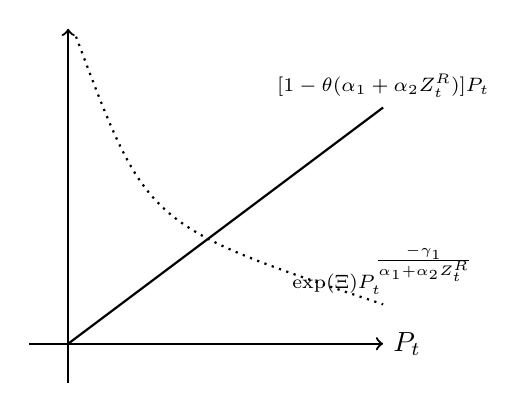
\begin{tikzpicture}
            \draw[->,thick] (-0.5,0)--(4,0) node[right]{$P_t$};
            \draw[->,thick] (0,-0.5)--(0,4) ;
            \draw[dotted, thick] (0.1, 3.9) .. controls (1, 1.5)..(4,0.5) node[above]{\scriptsize{$\exp(\Xi) P_t^{\frac{-\gamma_1}{\alpha_1 + \alpha_2 Z^{R}_{t}}}$}};
            \draw[thick] (0,0) -- (4,3) node[above]{\scriptsize{$[1-\theta(\alpha_1+\alpha_2 Z_t^R)]P_t$}};
        \end{tikzpicture}
        \caption{$\frac{-\gamma_1}{\alpha_1 + \alpha_2 Z^{R}_{t}} < 0$}
        \label{fig:fixed_monotone_decreasing}
    \end{subfigure}
    \hfill
    \begin{subfigure}{0.45\textwidth}
        \begin{tikzpicture}
            \draw[->,thick] (-0.5,0)--(4,0) node[right]{$P_t$};
            \draw[->,thick] (0,-0.5)--(0,4) ;
            \draw[dotted, thick] (0,0) .. controls (1, 2.0)..(4,2.5);
            \draw[thick] (0,0) -- (4,3);
        \end{tikzpicture}
         \caption{$\frac{-\gamma_1}{\alpha_1 + \alpha_2 Z^{R}_{t}} \in [0,1)$}
         \label{fig:fixed_concave}
    \end{subfigure}
    
    \vspace{1em}
    \begin{subfigure}{0.45\textwidth}
        \begin{tikzpicture}
            \draw[->,thick] (-0.5,0)--(4,0) node[right]{$P_t$};
            \draw[->,thick] (0,-0.5)--(0,4) ;
            \draw[dotted, thick] (0,0) -- (4,3);
            \draw[thin] (0,0) -- (4,3);
        \end{tikzpicture}
         \caption{$\frac{-\gamma_1}{\alpha_1 + \alpha_2 Z^{R}_{t}} = 1, 1-\theta(\alpha_1+\alpha_2 Z_t^R) = \exp(\Xi) $}
         \label{fig:fixed_coinside}
    \end{subfigure}
    \hfill
    \begin{subfigure}{0.45\textwidth}
        \begin{tikzpicture}
            \draw[->,thick] (-0.5,0)--(4,0) node[right]{$P_t$};
            \draw[->,thick] (0,-0.5)--(0,4) ;
            \draw[dotted, thick] (0,0) -- (4,3.9);
            \draw[thin] (0,0) -- (4,3);
        \end{tikzpicture}
         \caption{$\frac{-\gamma_1}{\alpha_1 + \alpha_2 Z^{R}_{t}} = 1, 1-\theta(\alpha_1+\alpha_2 Z_t^R) \ne \exp(\Xi) $}
         \label{fig:fixed_parallel}
    \end{subfigure}
    \vspace{1em}
    \begin{subfigure}{0.4\textwidth}
        \begin{tikzpicture}
            \draw[->,thick] (-0.5,0)--(4,0) node[right]{$P_t$};
            \draw[->,thick] (0,-0.5)--(0,4) ;
            \draw[dotted, thick] (0,0) .. controls (2, 0.5)..(4,3.5);
            \draw[thin] (0,0) -- (4,3);
        \end{tikzpicture}
         \caption{$\frac{-\gamma_1}{\alpha_1 + \alpha_2 Z^{R}_{t}}> 1$}
         \label{fig:fixed_convex}
    \end{subfigure}
    
    \footnotesize
    Note: As there is no equilibrium when $1- \theta(\alpha_1 + \alpha_2 Z^{R}_{t}) \le 0$, the above figures assume that $1- \theta(\alpha_1 + \alpha_2 Z^{R}_{t}) > 0$.
    The thick line represents the first term and the dotted line represents the second term in \eqref{eq:fixed_point}.
\end{figure}


From $\Delta (P_t) = 0$, the positive equilibrium price can be written as 
\begin{align}
    0 & = [1-\theta(\alpha_1 + \alpha_2 Z^{R}_{t})]P_t - \exp(\Xi) P_t^{\frac{-\gamma_1}{\alpha_1 + \alpha_2 Z^{R}_{t}}}\nonumber \\ 
    0 & = 1-\theta(\alpha_1 + \alpha_2 Z^{R}_{t}) - \exp(\Xi)P_t^{\frac{-\gamma_1}{\alpha_1 + \alpha_2 Z^{R}_{t}}- 1} \nonumber\\ 
    P_t^{\frac{-\gamma_1}{\alpha_1 + \alpha_2 Z^{R}_{t}}- 1} & = \frac{1-\theta(\alpha_1 + \alpha_2 Z^{R}_{t})}{ \exp(\Xi)}\nonumber\\ 
    P_{t}^* &= \left(\frac{1-\theta(\alpha_1 + \alpha_2 Z^{R}_{t})}{\exp(\Xi)}\right)^{-\frac{\alpha_1 + \alpha_2 Z^{R}_{t}}{\gamma_1 +\alpha_1 + \alpha_2 Z^{R}_{t}}}.
\end{align} 

Figure \ref{fg:equilibrium_existence_demand_supply} illustrates how the demand and supply equations cross under the conditions.
When $1- \theta(\alpha_1 + \alpha_2 Z^{R}_{t}) \le 0$, the supply equation \eqref{eq:log_linear_supply_equation} is ill-defined because the inside of the log function becomes negative.
Thus, there should not be any equilibrium.
Hereafter, assume that $1- \theta(\alpha_1 + \alpha_2 Z^{R}_{t}) > 0$.
When $-\gamma_1/(\alpha_1 + \alpha_2 Z^{R}_{t}) = 1$ and $\exp(\Xi) = 1- \theta(\alpha_1 + \alpha_2 Z^{R}_{t})$, the demand equation and supply equation coincides.
Thus there are infinitely many equilibria in the model.
When $-\gamma_1/(\alpha_1 + \alpha_2 Z^{R}_{t}) = 1$ and $\exp(\Xi) \ne 1- \theta(\alpha_1 + \alpha_2 Z^{R}_{t})$, the demand and supply equations have a same slope and different intercepts, which means that both equations become parallel.
Thus, there is no equilibrium.
When $-\gamma_1/(\alpha_1 + \alpha_2 Z^{R}_{t}) \ne 1$, the demand and supply equations have different slopes, and hence we can find a unique equilibrium. 


\begin{figure}[!ht]
    \caption{The illustrations of the equilibrium existence}
    \label{fg:equilibrium_existence_demand_supply}
    \begin{subfigure}{0.45\textwidth}
        \begin{tikzpicture}
            \draw[->,thick] (-0.5,0)--(4,0) node[right]{$Q_t$};
            \draw[->,thick] (0,-0.5)--(0,4) node[above]{$P_t$};
            \draw[blue, thick] (0,0.5) .. controls (1, 2.2)..(4,3) node[right]{$S$};
            \draw[red, thin] (0,0.5) .. controls (1, 2.2)..(4,3) node[above]{$D$};
        \end{tikzpicture}
         \caption{$-\gamma_1/(\alpha_1 + \alpha_2 Z^{R}_{t}) = 1$ and $\exp(\Xi) = 1- \theta(\alpha_1 + \alpha_2 Z^{R}_{t})$}
    \end{subfigure}
    \hfill
    \begin{subfigure}{0.45\textwidth}
        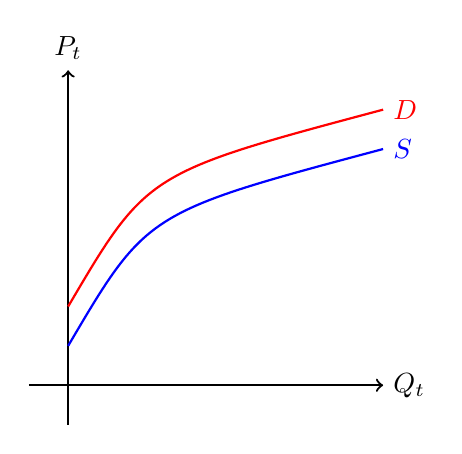
\begin{tikzpicture}
            \draw[->,thick] (-0.5,0)--(4,0) node[right]{$Q_t$};
            \draw[->,thick] (0,-0.5)--(0,4) node[above]{$P_t$};
            \draw[blue, thick] (0, 0.5) .. controls (1, 2.2)..(4,3) node[right]{$S$};
            \draw[red, thick, yshift = 5mm] (0, 0.5) .. controls (1, 2.2)..(4,3) node[right]{$D$};
        \end{tikzpicture}
        \caption{$-\gamma_1/(\alpha_1 + \alpha_2 Z^{R}_{t}) = 1$ and $\exp(\Xi) \ne 1- \theta(\alpha_1 + \alpha_2 Z^{R}_{t})$}
    \end{subfigure}
    
    \vspace{1em}
    \begin{subfigure}{0.45\textwidth}
        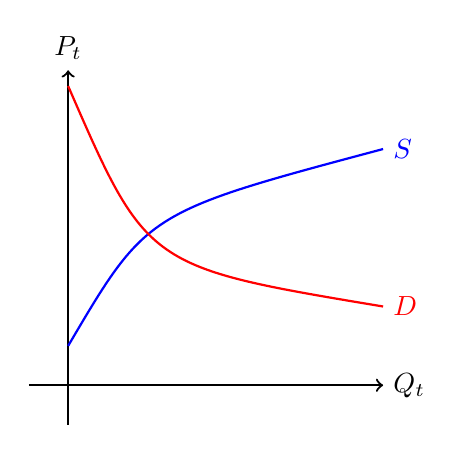
\begin{tikzpicture}
            \draw[->,thick] (-0.5,0)--(4,0) node[right]{$Q_t$};
            \draw[->,thick] (0,-0.5)--(0,4) node[above]{$P_t$};
            \draw[blue, thick] (0,0.5) .. controls (1, 2.2)..(4,3) node[right]{$S$};
            \draw[red, thick] (0,3.8) .. controls (1, 1.5) .. (4,1.0)  node[right]{$D$};
        \end{tikzpicture}
         \caption{$\gamma_1/(\alpha_1 + \alpha_2 Z^{R}_{t}) \ne 1$, $\alpha_1 + \alpha_2 Z^{R}_{t}>0$, and $\gamma_1>0$}
    \end{subfigure}
    \hfill
    \begin{subfigure}{0.45\textwidth}
        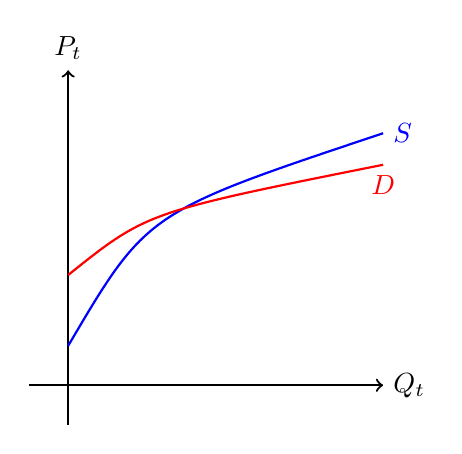
\begin{tikzpicture}
            \draw[->,thick] (-0.5,0)--(4,0) node[right]{$Q_t$};
            \draw[->,thick] (0,-0.5)--(0,4) node[above]{$P_t$};
            \draw[blue, thick] (0,0.5) .. controls (1, 2.2)..(4,3.2) node[right]{$S$};
            \draw[red, thick] (0,1.4) .. controls (1, 2.2) .. (4,2.8)  node[below]{$D$};
        \end{tikzpicture}
         \caption{$\gamma_1/(\alpha_1 + \alpha_2 Z^{R}_{t}) \ne 1$, $\alpha_1 + \alpha_2 Z^{R}_{t}\le0$, and $\gamma_1>0$}
    \end{subfigure}
    \vspace{1em}
    \begin{subfigure}{0.45\textwidth}
        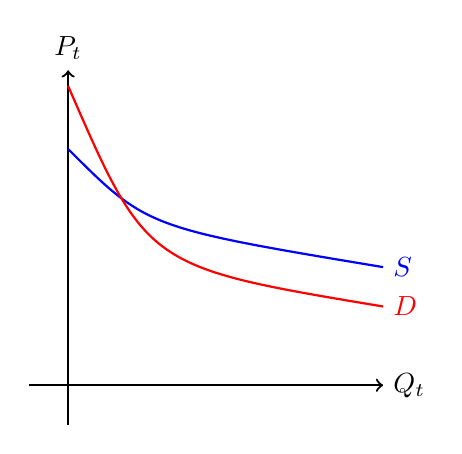
\begin{tikzpicture}
            \draw[->,thick] (-0.5,0)--(4,0) node[right]{$Q_t$};
            \draw[->,thick] (0,-0.5)--(0,4) node[above]{$P_t$};
            \draw[blue, thick] (0,3.0) .. controls (1, 2.0)..(4,1.5) node[right]{$S$};
            \draw[red, thick] (0,3.8) .. controls (1, 1.5) .. (4,1.0)  node[right]{$D$};
        \end{tikzpicture}
         \caption{$\gamma_1/(\alpha_1 + \alpha_2 Z^{R}_{t}) \ne 1$, $\alpha_1 + \alpha_2 Z^{R}_{t}>0$, and $\gamma_1\le 0$}
    \end{subfigure}
    \hfill
    \begin{subfigure}{0.45\textwidth}
        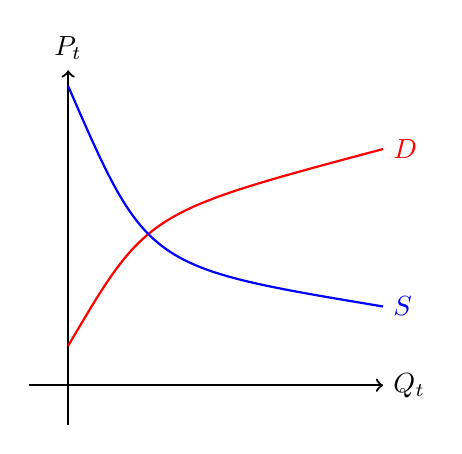
\begin{tikzpicture}
            \draw[->,thick] (-0.5,0)--(4,0) node[right]{$Q_t$};
            \draw[->,thick] (0,-0.5)--(0,4) node[above]{$P_t$};
            \draw[red, thick] (0,0.5) .. controls (1, 2.2)..(4,3) node[right]{$D$};
            \draw[blue, thick] (0,3.8) .. controls (1, 1.5) .. (4,1.0)  node[right]{$S$};
        \end{tikzpicture}
         \caption{$\gamma_1/(\alpha_1 + \alpha_2 Z^{R}_{t}) \ne 1$, $\alpha_1 + \alpha_2 Z^{R}_{t}\le 0$, and $\gamma_1\le 0$}
    \end{subfigure}
    
    \footnotesize
    Note: As there is no equilibrium when $1- \theta(\alpha_1 + \alpha_2 Z^{R}_{t}) \le 0$, the above figures assume that $1- \theta(\alpha_1 + \alpha_2 Z^{R}_{t}) > 0$. 
    %Case (a) considers the case $-\gamma_1/(\alpha_1 + \alpha_2 Z^{R}_{t}) = 1$ and $\exp(\Xi) = 1- \theta(\alpha_1 + \alpha_2 Z^{R}_{t})$. Case (b) considers the case $-\gamma_1/(\alpha_1 + \alpha_2 Z^{R}_{t}) = 1$ and $\exp(\Xi) \ne 1- \theta(\alpha_1 + \alpha_2 Z^{R}_{t})$.
    %Case (c), (d), (e), and (f) consider the case $\gamma_1/(\alpha_1 + \alpha_2 Z^{R}_{t}) \ne 1$.
    Case (a) and (b) also allow both the demand and supply equations to be downward sloping.
\end{figure}







\newpage


\subsection{Simulation and estimation procedure}\label{sec:setting}
We assess the performance of the MPEC estimator using Monte Carlo simulation.
To generate the simulation data, for each model, we first generate the exogenous variables $Y_t, Z^{R}_{t}, W_t, R_{t}, H_t$, and $K_t$ and the error terms $\varepsilon_{t}^c$ and $\varepsilon_{t}^d$ based on the data generation process in Table \ref{tb:parameter_setting}.
By substituting the Equation \eqref{eq:log_linear_demand} into Equation \eqref{eq:log_linear_supply_equation} and solving it for $P_{t}$, the log aggregate quantity is given as: 
\begin{align}
    \log Q_t &= \frac{ \alpha_0 + \alpha_3 \log Y_t + \log (1 - \theta (\alpha_1 + \alpha_2 Z^{R}_{t})) - \gamma_0  -  \gamma_2 \log W_{t} - \gamma_3 \log R_t + \varepsilon^{d}_{t} - \varepsilon^{c}_{t}}{\gamma_1+ \alpha_1 + \alpha_2 Z^{R}_{t} }.\label{eq:quantity_loglinear}
\end{align}
We compute the equilibrium quantity $Q_{t}$ for the log-linear model by \eqref{eq:quantity_loglinear}.
We then compute the equilibrium price $P_t$ by substituting $Q_{t}$ and other variables into the demand function \eqref{eq:log_linear_demand}.
We generate 1000 data sets of 100, 200, 1000, 1500 markets.
We jointly estimate the demand and supply parameters by the simultaneous equation model \citep{wooldridge2010econometric} from the true values.
The instrument variables for the demand estimation are $Z^{d}_{t} = (1, Z^{R}_{t}, \log Y_t, H_{t}, K_{t})^\top$ and the instrument variables for the supply estimation are $Z^{c}_{t} = (1, Z^{R}_{t}, \log W_{t}, \log R_{t}, \log Y_t)^\top$. 
We use state-of-the-art constrained optimization solvers, i.e., \texttt{Ipopt.jl} which implements an interior point line search filter method that aims to find a local solution of nonlinear programming problems.
Note that derivative-free algorithms such as Nelder-Mead algorithm cannot properly finish the optimization routine to solve the model because the above log-transformation problem arises even if the parameter search starts from the true values.
We use the following weight matrix:
\begin{align}
    W = \left[\frac{1}{T}\sum_{t = 1}^T Z_t^\top Z_t\right]^{-1} \text{ where } Z_{t}=\left[\begin{array}{ll}
        Z_{t}^{d\top} & 0 \\
        0 & Z_{t}^{c\top}
    \end{array}\right].\label{eq:weight_matrix}
\end{align}


\begin{table}[!htbp]
    \caption{True parameters and distributions}
    \label{tb:parameter_setting}
    \begin{center}
    \subfloat[Parameters]{
    \begin{tabular}{crr}
            \hline
            $\alpha_0$  & $20.0$ &\\
            $\alpha_1$ & $1.0$  &\\
            $\alpha_2$ & $0.1$ &\\
            $\alpha_3$ & $1.0$ &\\
            $\gamma_0$ & $5.0$  &\\
            $\gamma_1$ & $1.0$  &\\
            $\gamma_2$ & $1.0$ &\\
            $\gamma_3$ & $1.0$ &\\
            $\theta$ & $0.5$  &\\
            \hline
        \end{tabular}
    }
    \subfloat[Distributions]{
    \begin{tabular}{crr}
            \hline
            Demand shifter&  &  \\
            $Y_t$ & $N(0,1)$ \\
            Demand rotation instrument&  &  \\
            $Z^{R}_{t}$ & $U(0,1)$ \\
            Cost shifter  &  \\
            $W_{t}$ & $U(1,3)$ \\
            $R_t$  & $U(1,3)$  \\
            $H_{t}$ & $W_{t}+U(0,1)$  \\
            $K_{t}$ & $R_{t}+U(0,1)$  \\
            Error&  &  \\
            $\varepsilon^{d}_{t}$ & $N(0,\sigma)$  \\
            $\varepsilon^{c}_{t}$ & $N(0,\sigma)$ \\
            \hline
        \end{tabular}
    }
    \end{center}
    \footnotesize
    Note: $\sigma=\{0.5, 1.0, 2.0\}$. $N:$ Normal distribution. $U:$ Uniform distribution.
\end{table}


\subsection{Nonlinear system of 2SLS estimator}\label{sec:n2sls}
Given the demand equation \eqref{eq:log_linear_demand} and the supply equation \eqref{eq:log_linear_supply_equation}, we can write the error terms in the demand and supply equation as
\begin{align}
    {\varepsilon}_t^d(\xi) & =  \log P_{t} - \alpha_0 + (\alpha_1 + \alpha_2 Z^{R}_{t}) \log Q_t - \alpha_3 \log Y_t \label{eq:residual_demand_2sls}, \\
    {\varepsilon}_t^c(\xi) & =  \log P_t + \log(1 - \theta(\alpha_1 + \alpha_2 Z^{R}_{t})) -\gamma_0 - \gamma_1 \log Q_t -  \gamma_2 \log W_{t} -\gamma_3 \log R_t \label{eq:residual_supply_2sls}.
\end{align}
To estimate the parameters, we convert the conditional moment conditions, $E[\varepsilon_t^d\mid Z_t^d] = E[\varepsilon_t^c\mid Z_t^c]=0$, into unconditional moment conditions, $E[\varepsilon_t^d Z_t^d] = E[\varepsilon_t^cZ_t^c]=0$.
Using Equations \eqref{eq:residual_demand_2sls} and \eqref{eq:residual_supply_2sls}, we construct the sample analog of the moment conditions:
\begin{align*}
    g(\xi) = \left[\begin{array}{l}
    \frac{1}{T}\sum_{t=1}^T{\varepsilon}^{d}_{t}(\xi)Z_{t}^{d} \\
    \frac{1}{T}\sum_{t=1}^T{\varepsilon}^{c}_{t}(\xi)Z_{t}^{c}
    \end{array}\right].
\end{align*}
For some weighting matrix $W$, we define the GMM estimator as the vector $\xi^*$ that solves the problem,
\begin{align}
    \min_{\xi}\ g(\xi)^\top W g(\xi) \label{eq:minimization_gmm}. 
\end{align}
When we use the weight matrix \eqref{eq:weight_matrix}, the solution to \eqref{eq:minimization_gmm} is called the nonlinear system 2SLS estimator (N2SLS). 
We emphasize that the primary distinction between the MPEC and 2SLS estimators lies in the construction of the supply residuals. 
This means that while the MPEC estimator circumvents the log-transformation problem by treating the first-order condition as an equality constraint and considering $MC_t$ as a variable for the minimization problem, N2SLS encounters the log-transformation problem when using \eqref{eq:residual_supply_2sls}.


\subsection{Additional experiments}\label{sec:additional_experiments}

Tables \ref{tab:unnamed-chunk-13} and \ref{tab:unnamed-chunk-22} compare MPEC and N2SLS in 1,000 datasets, examining convergence and the GMM objective value. 
We illustrate this with $T=1500$ and $\sigma=1.0$ compared to $T=100$ and $\sigma=1.0$ in the main text. 
If the absolute parameter difference between N2SLS and MPEC for at least one parameter exceeds 1e-2, we label it as ``different sol." When the GMM objective value difference is less than 1e-4, we label it as ``same obj." 
In small samples ($T=100$), MPEC outperforms N2SLS in GMM objective function for 37.8\% of datasets, while N2SLS is better in 24.6\%. 
This suggests MPEC is not clearly superior in small samples. 
However, in large samples ($T=1500$), MPEC beats N2SLS in GMM objective function for 76.5\% of datasets, with N2SLS better in 23.0\%. 
This implies that MPEC is better than N2SLS but not perfect in large samples, using the same starting values as true values.
These results are robust to tolerance levels and $\sigma$ choices. 

\begin{table}
\centering
\begin{talltblr}[         %% tabularray outer open
caption={Fraction of convergence and smaller GMM objective value (\$T=100,\textbackslash{}sigma=1.0\$)},
]                     %% tabularray outer close
{                     %% tabularray inner open
colspec={Q[]Q[]Q[]},
column{1}={}{halign=l,},
column{2,3}={}{halign=r,},
}                     %% tabularray inner close
\toprule
classification & N & \% \\ \midrule %% TinyTableHeader
Both converged, different sol, MPEC has lower obj  & 378 & 37.8 \\
Both converged, different sol, N2SLS has lower obj & 246 & 24.6 \\
Both converged, different sol, same obj            & 16  & 1.6  \\
Both converged, same sol                           & 356 & 35.6 \\
MPEC only converged                                & 4   & 0.4  \\
\bottomrule
\end{talltblr}
\end{table}


\begin{table}
\centering
\begin{talltblr}[         %% tabularray outer open
caption={Fraction of convergence and smaller GMM objective value (\$T=1500,\textbackslash{}sigma=1.0\$)},
]                     %% tabularray outer close
{                     %% tabularray inner open
colspec={Q[]Q[]Q[]},
column{1}={}{halign=l,},
column{2,3}={}{halign=r,},
}                     %% tabularray inner close
\toprule
classification & N & \% \\ \midrule %% TinyTableHeader
Both converged, different sol, MPEC has lower obj  & 765 & 76.5 \\
Both converged, different sol, N2SLS has lower obj & 230 & 23.0 \\
Both converged, different sol, same obj            & 5   & 0.5  \\
\bottomrule
\end{talltblr}
\end{table}


Table \ref{tb:loglinear_loglinear_sigma_1_mpec_theta_constraint_slope_constraint_bias_rmse} compares MPEC estimation with N2SLS estimation with and without Constraints \eqref{eq:slope_constraint} and \eqref{eq:equlibrium_existence} by adding an extra table to the main text.
Additional results for different $\sigma$ are shown in Tables \ref{tb:loglinear_loglinear_sigma_0.5_mpec_non_constraint_theta_constraint} and \ref{tb:loglinear_loglinear_sigma_2_mpec_non_constraint_theta_constraint}. 
As a summary, the main findings in the main text are robust.

Table \ref{tb:loglinear_loglinear_sigma_1_simultaneous_non_constraint_non_constraint_bias_rmse} shows that N2SLS without all constraints searches parameters in the domain where no equilibrium exists and obtains implausible estimated parameters.
Thus, Constraint \eqref{eq:conduct_constraint} is crucial in estimating the model.

\begin{table}[!htbp]
  \begin{center}
      \caption{Performance comparison}
      \label{tb:loglinear_loglinear_sigma_1_mpec_theta_constraint_slope_constraint_bias_rmse} 
      % \subfloat[Separate]{
\begin{tabular}[t]{llrrrrrrr}
\toprule
  & Bias & RMSE & Bias & RMSE & Bias & RMSE & Bias & RMSE\\
\midrule
$\alpha_{0}$ & -0.442 & 1.669 & -0.122 & 0.943 & -0.017 & 0.612 & 0.007 & 0.267\\
$\alpha_{1}$ & -0.246 & 0.949 & -0.071 & 0.529 & -0.013 & 0.348 & 0.005 & 0.151\\
$\alpha_{2}$ & 0.022 & 0.173 & 0.013 & 0.106 & 0.006 & 0.068 & -0.001 & 0.030\\
$\alpha_{3}$ & -0.109 & 0.544 & -0.030 & 0.297 & -0.007 & 0.205 & 0.003 & 0.090\\
$\gamma_{0}$ & -0.356 & 1.739 & -0.321 & 1.248 & -0.200 & 0.855 & -0.031 & 0.388\\
$\gamma_{1}$ & 0.088 & 0.516 & 0.060 & 0.350 & 0.039 & 0.236 & 0.006 & 0.096\\
$\gamma_{2}$ & 0.040 & 0.399 & 0.035 & 0.260 & 0.024 & 0.172 & 0.004 & 0.073\\
$\gamma_{3}$ & 0.042 & 0.391 & 0.035 & 0.262 & 0.021 & 0.179 & 0.003 & 0.077\\
$\theta$ & 0.125 & 0.409 & 0.120 & 0.363 & 0.068 & 0.285 & 0.000 & 0.163\\
Runs converged (\%) &  & 97.400 &  & 98.300 &  & 98.900 &  & 100.000\\
Sample size ($T$) &  & 50 &  & 100 &  & 200 &  & 1000\\
\bottomrule
\end{tabular}
}\\
    \subfloat[N2SLS with Constraints \eqref{eq:slope_constraint} and \eqref{eq:equlibrium_existence}]{
\begin{tabular}[t]{lrrrrrrrr}
\toprule
  & Bias & RMSE & Bias & RMSE & Bias & RMSE & Bias & RMSE\\
\midrule
$\alpha_{0}$ & -1.922 & 8.603 & -0.068 & 5.116 & 0.037 & 2.035 & 0.000 & 1.556\\
$\alpha_{1}$ & -0.299 & 1.314 & -0.010 & 0.785 & 0.005 & 0.312 & 0.000 & 0.240\\
$\alpha_{2}$ & -0.013 & 0.104 & -0.002 & 0.063 & 0.001 & 0.024 & 0.000 & 0.019\\
$\alpha_{3}$ & -0.165 & 0.774 & -0.007 & 0.472 & -0.004 & 0.185 & -0.001 & 0.152\\
$\gamma_{0}$ & -1.767 & 14.394 & -1.001 & 6.530 & -0.208 & 1.993 & -0.156 & 1.566\\
$\gamma_{1}$ & 0.255 & 1.949 & 0.132 & 0.838 & 0.034 & 0.229 & 0.027 & 0.174\\
$\gamma_{2}$ & 0.125 & 1.097 & 0.053 & 0.475 & 0.017 & 0.150 & 0.019 & 0.119\\
$\gamma_{3}$ & 0.099 & 0.903 & 0.062 & 0.481 & 0.007 & 0.149 & 0.014 & 0.120\\
$\theta$ & -0.098 & 0.441 & -0.060 & 0.421 & -0.061 & 0.319 & -0.058 & 0.281\\
Runs converged (\%) &  & 98.100 &  & 98.700 &  & 100.000 &  & 100.000\\
Sample size ($T$) &  & 100 &  & 200 &  & 1000 &  & 1500\\
\bottomrule
\end{tabular}
}\\
    \subfloat[N2SLS with Constraints \eqref{eq:conduct_constraint}, \eqref{eq:slope_constraint}, and \eqref{eq:equlibrium_existence}]{
\begin{tabular}[t]{llrrrrrrr}
\toprule
  & Bias & RMSE & Bias & RMSE & Bias & RMSE & Bias & RMSE\\
\midrule
$\alpha_{0}$ & -0.905 & 6.954 & 0.120 & 5.001 & 0.072 & 2.042 & 0.052 & 1.563\\
$\alpha_{1}$ & -0.141 & 1.053 & 0.018 & 0.768 & 0.010 & 0.313 & 0.008 & 0.241\\
$\alpha_{2}$ & -0.006 & 0.101 & 0.000 & 0.062 & 0.001 & 0.024 & 0.001 & 0.019\\
$\alpha_{3}$ & -0.088 & 0.620 & 0.007 & 0.475 & -0.001 & 0.186 & 0.003 & 0.152\\
$\gamma_{0}$ & -1.748 & 14.206 & -0.938 & 6.428 & 0.015 & 1.995 & 0.163 & 1.570\\
$\gamma_{1}$ & 0.254 & 1.927 & 0.129 & 0.825 & 0.018 & 0.226 & 0.003 & 0.170\\
$\gamma_{2}$ & 0.117 & 1.083 & 0.049 & 0.467 & 0.008 & 0.148 & 0.007 & 0.116\\
$\gamma_{3}$ & 0.098 & 0.890 & 0.058 & 0.478 & -0.001 & 0.148 & 0.003 & 0.118\\
$\theta$ & -0.100 & 0.441 & -0.072 & 0.424 & -0.121 & 0.351 & -0.148 & 0.333\\
Runs converged (\%) &  & 99.600 &  & 99.900 &  & 100.000 &  & 100.000\\
Sample size ($T$) &  & 100 &  & 200 &  & 1000 &  & 1500\\
\bottomrule
\end{tabular}
}\\
    \subfloat[MPEC ]{
\begin{tabular}[t]{lrrrrrrrr}
\toprule
  & Bias & RMSE & Bias & RMSE & Bias & RMSE & Bias & RMSE\\
\midrule
$\alpha_{0}$ & -0.614 & 5.995 & -0.213 & 4.315 & 0.077 & 2.034 & 0.063 & 1.555\\
$\alpha_{1}$ & -0.085 & 0.902 & -0.024 & 0.663 & 0.011 & 0.312 & 0.010 & 0.240\\
$\alpha_{2}$ & -0.028 & 0.105 & -0.022 & 0.073 & 0.000 & 0.025 & 0.001 & 0.020\\
$\alpha_{3}$ & -0.070 & 0.549 & -0.019 & 0.431 & -0.001 & 0.185 & 0.004 & 0.152\\
$\gamma_{0}$ & -5.106 & 15.922 & -2.379 & 6.990 & -0.375 & 1.959 & -0.398 & 1.533\\
$\gamma_{1}$ & 0.386 & 2.047 & 0.141 & 0.839 & 0.045 & 0.229 & 0.044 & 0.175\\
$\gamma_{2}$ & 0.190 & 1.155 & 0.054 & 0.475 & 0.022 & 0.150 & 0.027 & 0.120\\
$\gamma_{3}$ & 0.163 & 1.006 & 0.065 & 0.482 & 0.013 & 0.149 & 0.023 & 0.121\\
$\theta$ & 0.186 & 0.442 & 0.158 & 0.422 & -0.007 & 0.275 & 0.014 & 0.217\\
Runs converged (\%) &  & 100.000 &  & 100.000 &  & 100.000 &  & 100.000\\
Sample size ($T$) &  & 100 &  & 200 &  & 1000 &  & 1500\\
\bottomrule
\end{tabular}
}\\
  \end{center}
  \footnotesize
  Note: The error terms are drawn from a normal distribution, $N(0, \sigma)$. True values: $\alpha_0=20.0,\alpha_1=1.0,\alpha_2=0.1,\alpha_3=1.0,\gamma_0=5.0,\gamma_1=1.0,\gamma_2=1.0,\gamma_3=1.0,\theta=0.5$ and $\sigma=1.0$.
\end{table} 



% \subsection{Standard Estimation Methods}
% We summarize the results of the standard estimation using a derivative-free optimization algorithm such as Nelder-Mead algorithm and the standard estimation using state-of-the-art constrained optimization solvers, i.e., \texttt{Ipopt.jl} which implements an interior point line search filter method that aims to find a local solution of nonlinear programming problems. 
% First, as mentioned in the main text, the standard simultaneous equation approach using derivative-free algorithms such as Nelder-Mead algorithm could not properly finish the optimization routine to solve the model because the above log-transformation problem arises even if the parameter search starts from the true values. 
% Second, we examine the Two-Stage-Least-Square (2SLS) model in which Ipopt is implemented for minimizing only its supply side moments and the simultaneous equation model in which Ipopt is implemented for minimizing both demand and supply side moments. 
% We refer to the former as separate estimation and the latter as simultaneous estimation.
% These two estimation procedures are considered to be a middle ground between MPEC and standard approaches because these do not use equilibrium constraints but state-of-the-art constrained optimization
% solvers.

% Tables \ref{tb:loglinear_loglinear_sigma_2_separate_non_constraint_theta_constraint_bias_rmse} and \ref{tb:loglinear_loglinear_sigma_1_simultaneous_non_constraint_theta_constraint_bias_rmse} shows that both estimations fail in estimation for about 1\% of the simulation samples even if the parameter search starts from the true values. 
% Also, if $\sigma=2.0$ and $T=1000$, RMSEs are more than 10 for three parameters. Thus, MPEC is better than these approaches even for the typical and simple log-linear model. 



% \begin{table}[!htbp]
%   \begin{center}
%       \caption{MPEC vs standard approaches ($\sigma=0.5$)}
%       \label{tb:loglinear_loglinear_sigma_0.5_separate_non_constraint_theta_constraint_bias_rmse} 
%       \subfloat[MPEC]{
\begin{tabular}[t]{llrrrrrrr}
\toprule
  & Bias & RMSE & Bias & RMSE & Bias & RMSE & Bias & RMSE\\
\midrule
$\alpha_{0}$ & -0.250 & 1.106 & -0.060 & 1.013 & 0.013 & 0.848 & -0.027 & 0.352\\
$\alpha_{1}$ & -0.146 & 0.642 & -0.040 & 0.568 & 0.004 & 0.481 & -0.015 & 0.203\\
$\alpha_{2}$ & 0.006 & 0.109 & 0.011 & 0.098 & 0.008 & 0.072 & -0.001 & 0.030\\
$\alpha_{3}$ & -0.057 & 0.431 & -0.015 & 0.316 & 0.003 & 0.266 & -0.007 & 0.114\\
$\gamma_{0}$ & -0.285 & 1.798 & -0.124 & 1.224 & -0.061 & 0.837 & 0.062 & 0.402\\
$\gamma_{1}$ & 0.036 & 0.566 & 0.034 & 0.384 & 0.018 & 0.246 & -0.001 & 0.104\\
$\gamma_{2}$ & 0.007 & 0.381 & 0.017 & 0.258 & 0.011 & 0.165 & 0.000 & 0.073\\
$\gamma_{3}$ & 0.017 & 0.393 & 0.021 & 0.262 & 0.009 & 0.175 & -0.001 & 0.077\\
$\theta$ & 0.066 & 0.356 & -0.019 & 0.285 & -0.027 & 0.245 & -0.061 & 0.187\\
Runs converged (\%) &  & 100.000 &  & 100.000 &  & 100.000 &  & 100.000\\
Sample size ($T$) &  & 50 &  & 100 &  & 200 &  & 1000\\
\bottomrule
\end{tabular}
}\\
%       % \subfloat[Separate]{
\begin{tabular}[t]{llrrrrrrr}
\toprule
  & Bias & RMSE & Bias & RMSE & Bias & RMSE & Bias & RMSE\\
\midrule
$\alpha_{0}$ & 0.000 & 0.004 & -0.002 & 0.004 & 0.001 & 0.002 & 0.000 & 0.001\\
$\alpha_{1}$ & 0.000 & 0.001 & -0.001 & 0.001 & 0.000 & 0.001 & 0.000 & 0.000\\
$\alpha_{2}$ & 0.000 & 0.000 & 0.000 & 0.000 & 0.000 & 0.000 & 0.000 & 0.000\\
$\alpha_{3}$ & 0.000 & 0.000 & 0.000 & 0.000 & 0.000 & 0.000 & 0.000 & 0.000\\
$\gamma_{0}$ & 0.000 & 0.006 & 0.003 & 0.005 & -0.001 & 0.003 & -0.001 & 0.001\\
$\gamma_{1}$ & 0.000 & 0.001 & 0.000 & 0.001 & 0.000 & 0.000 & 0.000 & 0.000\\
$\gamma_{2}$ & 0.000 & 0.001 & 0.000 & 0.000 & 0.000 & 0.000 & 0.000 & 0.000\\
$\gamma_{3}$ & 0.000 & 0.001 & 0.000 & 0.000 & 0.000 & 0.000 & 0.000 & 0.000\\
$\theta$ & -0.001 & 0.003 & -0.001 & 0.002 & 0.000 & 0.001 & 0.000 & 0.001\\
Runs converged (\%) &  & 100.000 &  & 100.000 &  & 100.000 &  & 100.000\\
Sample size ($T$) &  & 50 &  & 100 &  & 200 &  & 1000\\
\bottomrule
\end{tabular}
}\\
%     \subfloat[Simultaneous]{
\begin{tabular}[t]{llrrrrrrr}
\toprule
  & Bias & RMSE & Bias & RMSE & Bias & RMSE & Bias & RMSE\\
\midrule
$\alpha_{0}$ & -0.207 & 2.884 & -0.033 & 1.089 & 0.039 & 0.852 & 0.007 & 0.265\\
$\alpha_{1}$ & -0.113 & 1.605 & -0.022 & 0.614 & 0.019 & 0.482 & 0.005 & 0.150\\
$\alpha_{2}$ & -0.015 & 0.169 & 0.007 & 0.109 & 0.008 & 0.075 & -0.001 & 0.029\\
$\alpha_{3}$ & -0.053 & 0.661 & -0.006 & 0.331 & 0.009 & 0.266 & 0.003 & 0.090\\
$\gamma_{0}$ & -0.778 & 2.847 & -0.554 & 2.430 & -0.322 & 1.088 & -0.089 & 0.470\\
$\gamma_{1}$ & 0.149 & 0.846 & 0.095 & 0.832 & 0.034 & 0.258 & 0.006 & 0.105\\
$\gamma_{2}$ & 0.069 & 0.544 & 0.048 & 0.450 & 0.019 & 0.171 & 0.003 & 0.074\\
$\gamma_{3}$ & 0.074 & 0.540 & 0.049 & 0.387 & 0.017 & 0.180 & 0.002 & 0.078\\
$\theta$ & 0.135 & 0.411 & 0.108 & 0.373 & 0.082 & 0.330 & 0.022 & 0.215\\
Runs converged (\%) &  & 99.000 &  & 98.700 &  & 99.800 &  & 100.000\\
Sample size ($T$) &  & 50 &  & 100 &  & 200 &  & 1000\\
\bottomrule
\end{tabular}
}
%   \end{center}
%   \footnotesize
%   %Note: 
% \end{table} 

\begin{table}[!htbp]
  \begin{center}
      \caption{MPEC vs N2SLS ($\sigma=0.5$)}
      \label{tb:loglinear_loglinear_sigma_0.5_mpec_non_constraint_theta_constraint} 
      \subfloat[N2SLS with Constraints \eqref{eq:slope_constraint} and \eqref{eq:equlibrium_existence}]{
\begin{tabular}[t]{llrrrrrrr}
\toprule
  & Bias & RMSE & Bias & RMSE & Bias & RMSE & Bias & RMSE\\
\midrule
$\alpha_{0}$ & -0.087 & 3.688 & 0.145 & 3.117 & 0.027 & 0.975 & -0.066 & 0.764\\
$\alpha_{1}$ & -0.014 & 0.565 & 0.021 & 0.477 & 0.004 & 0.150 & -0.010 & 0.117\\
$\alpha_{2}$ & 0.001 & 0.045 & 0.003 & 0.036 & 0.000 & 0.012 & -0.001 & 0.010\\
$\alpha_{3}$ & -0.004 & 0.317 & 0.009 & 0.263 & 0.002 & 0.090 & -0.004 & 0.073\\
$\gamma_{0}$ & -0.679 & 3.764 & -0.257 & 2.192 & 0.015 & 0.984 & 0.040 & 0.815\\
$\gamma_{1}$ & 0.097 & 0.465 & 0.041 & 0.253 & 0.004 & 0.104 & 0.000 & 0.084\\
$\gamma_{2}$ & 0.049 & 0.290 & 0.023 & 0.170 & 0.002 & 0.073 & 0.003 & 0.060\\
$\gamma_{3}$ & 0.050 & 0.288 & 0.021 & 0.178 & 0.001 & 0.077 & 0.001 & 0.058\\
$\theta$ & -0.063 & 0.389 & -0.068 & 0.333 & -0.043 & 0.199 & -0.032 & 0.167\\
Runs converged (\%) &  & 99.500 &  & 99.700 &  & 100.000 &  & 100.000\\
Sample size ($T$) &  & 100 &  & 200 &  & 1000 &  & 1500\\
\bottomrule
\end{tabular}
}\\
    \subfloat[N2SLS with Constraints \eqref{eq:conduct_constraint}, \eqref{eq:slope_constraint}, and \eqref{eq:equlibrium_existence}]{
\begin{tabular}[t]{lrrrrrrrr}
\toprule
  & Bias & RMSE & Bias & RMSE & Bias & RMSE & Bias & RMSE\\
\midrule
$\alpha_{0}$ & -0.006 & 3.556 & 0.175 & 3.158 & 0.059 & 0.977 & -0.017 & 0.763\\
$\alpha_{1}$ & -0.002 & 0.545 & 0.026 & 0.484 & 0.009 & 0.150 & -0.003 & 0.117\\
$\alpha_{2}$ & 0.002 & 0.044 & 0.004 & 0.037 & 0.000 & 0.012 & 0.000 & 0.010\\
$\alpha_{3}$ & 0.001 & 0.309 & 0.012 & 0.266 & 0.005 & 0.091 & 0.000 & 0.073\\
$\gamma_{0}$ & -0.616 & 3.317 & -0.221 & 2.191 & 0.275 & 1.076 & 0.421 & 0.972\\
$\gamma_{1}$ & 0.089 & 0.399 & 0.038 & 0.252 & -0.015 & 0.107 & -0.027 & 0.089\\
$\gamma_{2}$ & 0.044 & 0.265 & 0.022 & 0.170 & -0.007 & 0.074 & -0.011 & 0.061\\
$\gamma_{3}$ & 0.046 & 0.273 & 0.019 & 0.178 & -0.008 & 0.078 & -0.012 & 0.059\\
$\theta$ & -0.064 & 0.390 & -0.079 & 0.339 & -0.119 & 0.260 & -0.145 & 0.261\\
Runs converged (\%) &  & 99.900 &  & 100.000 &  & 100.000 &  & 100.000\\
Sample size ($T$) &  & 100 &  & 200 &  & 1000 &  & 1500\\
\bottomrule
\end{tabular}
}\\
    \subfloat[MPEC]{
\begin{tabular}[t]{llrrrrrrr}
\toprule
  & Bias & RMSE & Bias & RMSE & Bias & RMSE & Bias & RMSE\\
\midrule
$\alpha_{0}$ & -0.347 & 2.978 & -0.153 & 2.547 & 0.065 & 0.976 & -0.009 & 0.760\\
$\alpha_{1}$ & -0.043 & 0.452 & -0.016 & 0.388 & 0.010 & 0.150 & -0.001 & 0.117\\
$\alpha_{2}$ & -0.024 & 0.065 & -0.017 & 0.054 & 0.000 & 0.012 & 0.000 & 0.010\\
$\alpha_{3}$ & -0.028 & 0.265 & -0.013 & 0.224 & 0.005 & 0.091 & 0.001 & 0.073\\
$\gamma_{0}$ & -2.458 & 5.660 & -1.258 & 2.959 & -0.132 & 0.942 & -0.153 & 0.748\\
$\gamma_{1}$ & 0.112 & 0.602 & 0.057 & 0.260 & 0.014 & 0.103 & 0.014 & 0.082\\
$\gamma_{2}$ & 0.053 & 0.314 & 0.030 & 0.172 & 0.007 & 0.073 & 0.010 & 0.060\\
$\gamma_{3}$ & 0.061 & 0.426 & 0.028 & 0.181 & 0.006 & 0.077 & 0.008 & 0.058\\
$\theta$ & 0.169 & 0.407 & 0.109 & 0.356 & -0.003 & 0.155 & 0.017 & 0.116\\
Runs converged (\%) &  & 100.000 &  & 100.000 &  & 100.000 &  & 100.000\\
Sample size ($T$) &  & 100 &  & 200 &  & 1000 &  & 1500\\
\bottomrule
\end{tabular}
}
  \end{center}
  \footnotesize
  
\end{table} 

\begin{table}[!htbp]
  \begin{center}
      \caption{MPEC vs N2SLS ($\sigma=2.0$)}
      \label{tb:loglinear_loglinear_sigma_2_mpec_non_constraint_theta_constraint} 
      \subfloat[N2SLS with Constraints \eqref{eq:slope_constraint} and \eqref{eq:equlibrium_existence}]{
\begin{tabular}[t]{lrrrrrrrr}
\toprule
  & Bias & RMSE & Bias & RMSE & Bias & RMSE & Bias & RMSE\\
\midrule
$\alpha_{0}$ & -4.309 & 16.220 & -2.888 & 12.102 & -0.143 & 5.650 & 0.085 & 3.693\\
$\alpha_{1}$ & -0.657 & 2.489 & -0.448 & 1.840 & -0.024 & 0.874 & 0.012 & 0.568\\
$\alpha_{2}$ & -0.035 & 0.178 & -0.023 & 0.170 & 0.001 & 0.062 & 0.002 & 0.042\\
$\alpha_{3}$ & -0.280 & 1.174 & -0.250 & 1.181 & -0.027 & 0.545 & 0.003 & 0.323\\
$\gamma_{0}$ & 2.206 & 15.660 & -0.576 & 13.314 & -0.897 & 4.882 & -0.646 & 3.317\\
$\gamma_{1}$ & -0.255 & 2.096 & 0.100 & 1.753 & 0.119 & 0.607 & 0.086 & 0.399\\
$\gamma_{2}$ & -0.163 & 1.316 & 0.045 & 1.113 & 0.065 & 0.363 & 0.034 & 0.257\\
$\gamma_{3}$ & -0.155 & 1.669 & 0.068 & 1.127 & 0.061 & 0.386 & 0.041 & 0.271\\
$\theta$ & -0.201 & 0.474 & -0.142 & 0.463 & -0.053 & 0.400 & -0.050 & 0.374\\
Runs converged (\%) &  & 98.100 &  & 97.200 &  & 99.200 &  & 99.400\\
Sample size ($T$) &  & 100 &  & 200 &  & 1000 &  & 1500\\
\bottomrule
\end{tabular}
}\\
    \subfloat[N2SLS with Constraints \eqref{eq:conduct_constraint}, \eqref{eq:slope_constraint}, and \eqref{eq:equlibrium_existence}]{
\begin{tabular}[t]{llrrrrrrr}
\toprule
  & Bias & RMSE & Bias & RMSE & Bias & RMSE & Bias & RMSE\\
\midrule
$\alpha_{0}$ & -2.022 & 11.280 & -1.149 & 8.680 & 0.138 & 4.651 & 0.274 & 3.838\\
$\alpha_{1}$ & -0.310 & 1.771 & -0.181 & 1.313 & 0.019 & 0.712 & 0.041 & 0.590\\
$\alpha_{2}$ & -0.016 & 0.136 & -0.007 & 0.139 & 0.003 & 0.057 & 0.004 & 0.043\\
$\alpha_{3}$ & -0.148 & 0.984 & -0.113 & 0.875 & -0.003 & 0.428 & 0.017 & 0.333\\
$\gamma_{0}$ & 0.672 & 11.896 & -1.090 & 13.475 & -0.669 & 4.499 & -0.404 & 3.245\\
$\gamma_{1}$ & -0.046 & 1.598 & 0.172 & 1.770 & 0.098 & 0.556 & 0.066 & 0.391\\
$\gamma_{2}$ & -0.057 & 1.085 & 0.088 & 1.172 & 0.054 & 0.346 & 0.024 & 0.252\\
$\gamma_{3}$ & -0.020 & 1.204 & 0.108 & 1.225 & 0.050 & 0.365 & 0.031 & 0.267\\
$\theta$ & -0.229 & 0.475 & -0.163 & 0.464 & -0.088 & 0.410 & -0.108 & 0.394\\
Runs converged (\%) &  & 99.500 &  & 99.200 &  & 100.000 &  & 100.000\\
Sample size ($T$) &  & 100 &  & 200 &  & 1000 &  & 1500\\
\bottomrule
\end{tabular}
}\\
    \subfloat[MPEC]{
\begin{tabular}[t]{lrrrrrrrr}
\toprule
  & Bias & RMSE & Bias & RMSE & Bias & RMSE & Bias & RMSE\\
\midrule
$\alpha_{0}$ & -0.835 & 9.908 & -0.561 & 6.310 & 0.147 & 4.424 & 0.301 & 3.686\\
$\alpha_{1}$ & -0.109 & 1.563 & -0.076 & 0.935 & 0.024 & 0.677 & 0.047 & 0.566\\
$\alpha_{2}$ & -0.043 & 0.124 & -0.033 & 0.135 & -0.005 & 0.061 & 0.001 & 0.045\\
$\alpha_{3}$ & -0.047 & 0.909 & -0.078 & 0.664 & -0.004 & 0.404 & 0.018 & 0.323\\
$\gamma_{0}$ & -6.629 & 20.418 & -5.373 & 16.692 & -1.445 & 4.738 & -1.123 & 3.411\\
$\gamma_{1}$ & 0.422 & 2.630 & 0.384 & 2.103 & 0.137 & 0.580 & 0.115 & 0.409\\
$\gamma_{2}$ & 0.184 & 1.788 & 0.185 & 1.318 & 0.073 & 0.357 & 0.048 & 0.261\\
$\gamma_{3}$ & 0.199 & 1.885 & 0.215 & 1.496 & 0.068 & 0.376 & 0.055 & 0.276\\
$\theta$ & 0.225 & 0.459 & 0.227 & 0.447 & 0.098 & 0.357 & 0.084 & 0.313\\
Runs converged (\%) &  & 99.200 &  & 99.800 &  & 99.800 &  & 100.000\\
Sample size ($T$) &  & 100 &  & 200 &  & 1000 &  & 1500\\
\bottomrule
\end{tabular}
}
  \end{center}
  \footnotesize
  
\end{table} 


\begin{landscape}{
\begin{table}[!htbp]
  \begin{center}
      \caption{N2SLS without Constraints \eqref{eq:conduct_constraint}, \eqref{eq:slope_constraint}, and \eqref{eq:equlibrium_existence}}
      \label{tb:loglinear_loglinear_sigma_1_simultaneous_non_constraint_non_constraint_bias_rmse} 
      % \subfloat[$\sigma=0.5$]{
\begin{tabular}[t]{llrrrrrrr}
\toprule
  & Bias & RMSE & Bias & RMSE & Bias & RMSE & Bias & RMSE\\
\midrule
$\alpha_{0}$ & -0.250 & 1.106 & -0.060 & 1.013 & 0.013 & 0.848 & -0.027 & 0.352\\
$\alpha_{1}$ & -0.146 & 0.642 & -0.040 & 0.568 & 0.004 & 0.481 & -0.015 & 0.203\\
$\alpha_{2}$ & 0.006 & 0.109 & 0.011 & 0.098 & 0.008 & 0.072 & -0.001 & 0.030\\
$\alpha_{3}$ & -0.057 & 0.431 & -0.015 & 0.316 & 0.003 & 0.266 & -0.007 & 0.114\\
$\gamma_{0}$ & -0.285 & 1.798 & -0.124 & 1.224 & -0.061 & 0.837 & 0.062 & 0.402\\
$\gamma_{1}$ & 0.036 & 0.566 & 0.034 & 0.384 & 0.018 & 0.246 & -0.001 & 0.104\\
$\gamma_{2}$ & 0.007 & 0.381 & 0.017 & 0.258 & 0.011 & 0.165 & 0.000 & 0.073\\
$\gamma_{3}$ & 0.017 & 0.393 & 0.021 & 0.262 & 0.009 & 0.175 & -0.001 & 0.077\\
$\theta$ & 0.066 & 0.356 & -0.019 & 0.285 & -0.027 & 0.245 & -0.061 & 0.187\\
Runs converged (\%) &  & 100.000 &  & 100.000 &  & 100.000 &  & 100.000\\
Sample size ($T$) &  & 50 &  & 100 &  & 200 &  & 1000\\
\bottomrule
\end{tabular}
}\\
      \subfloat[N2SLS ($\sigma=0.5$)]{
\begin{tabular}[t]{llrrrrrrr}
\toprule
  & Bias & RMSE & Bias & RMSE & Bias & RMSE & Bias & RMSE\\
\midrule
$\alpha_{0}$ & 0.715 & 0.815 & 0.765 & 0.797 & 0.788 & 0.804 & 0.795 & 0.797\\
$\alpha_{1}$ & -0.169 & 0.900 & -0.066 & 0.514 & -0.018 & 0.337 & 0.005 & 0.118\\
$\alpha_{2}$ & -0.039 & 0.379 & -0.019 & 0.223 & -0.011 & 0.153 & -0.016 & 0.077\\
$\alpha_{3}$ & 0.707 & 1.047 & 0.794 & 0.941 & 0.834 & 0.900 & 0.855 & 0.864\\
$\gamma_{0}$ & 3.128 & 4.732 & 2.932 & 4.511 & 2.626 & 4.151 & 1.473 & 3.022\\
$\gamma_{1}$ & 0.040 & 0.302 & 0.015 & 0.194 & 0.005 & 0.130 & -0.001 & 0.056\\
$\gamma_{2}$ & 0.007 & 0.299 & 0.009 & 0.195 & 0.005 & 0.130 & 0.000 & 0.059\\
$\gamma_{3}$ & 0.018 & 0.173 & 0.008 & 0.110 & 0.002 & 0.075 & -0.001 & 0.033\\
$\theta$ & -1767.327 & 6217.525 & -1024.935 & 2976.989 & -751.215 & 2765.357 & -240.693 & 974.357\\
Runs converged (\%) &  & 99.000 &  & 98.500 &  & 99.100 &  & 98.700\\
Sample size ($T$) &  & 50 &  & 100 &  & 200 &  & 1000\\
\bottomrule
\end{tabular}
}\\
      % \subfloat[Separate]{
\begin{tabular}[t]{llrrrrrrr}
\toprule
  & Bias & RMSE & Bias & RMSE & Bias & RMSE & Bias & RMSE\\
\midrule
$\alpha_{0}$ & -1.209 & 2.406 & -0.848 & 2.098 & -0.337 & 1.188 & -0.014 & 0.512\\
$\alpha_{1}$ & -0.716 & 1.377 & -0.488 & 1.208 & -0.188 & 0.680 & -0.011 & 0.292\\
$\alpha_{2}$ & -0.044 & 0.307 & -0.024 & 0.202 & -0.021 & 0.133 & 0.000 & 0.056\\
$\alpha_{3}$ & -0.403 & 0.954 & -0.250 & 0.717 & -0.095 & 0.412 & -0.010 & 0.178\\
$\gamma_{0}$ & 4.537 & 7.248 & 3.715 & 8.543 & 3.653 & 4.268 & 3.735 & 3.838\\
$\gamma_{1}$ & -0.189 & 2.213 & 0.072 & 3.184 & 0.043 & 0.687 & 0.028 & 0.233\\
$\gamma_{2}$ & -0.098 & 1.046 & 0.018 & 1.049 & 0.013 & 0.453 & 0.014 & 0.152\\
$\gamma_{3}$ & -0.142 & 1.112 & 0.007 & 1.105 & 0.019 & 0.437 & 0.005 & 0.151\\
$\theta$ & 0.038 & 0.390 & 0.073 & 0.393 & 0.110 & 0.403 & 0.075 & 0.314\\
Runs converged (\%) &  & 95.600 &  & 94.900 &  & 93.500 &  & 99.100\\
Sample size ($T$) &  & 50 &  & 100 &  & 200 &  & 1000\\
\bottomrule
\end{tabular}
}\\
      \subfloat[N2SLS ($\sigma=1.0$)]{
\begin{tabular}[t]{llrrrrrrr}
\toprule
  & Bias & RMSE & Bias & RMSE & Bias & RMSE & Bias & RMSE\\
\midrule
$\alpha_{0}$ & -1.484 & 3.189 & -0.673 & 2.226 & NA & NA & NA & NA\\
$\alpha_{1}$ & -0.850 & 1.781 & -0.452 & 1.199 & NA & NA & NA & NA\\
$\alpha_{2}$ & -0.033 & 0.316 & 0.013 & 0.232 & NA & NA & NA & NA\\
$\alpha_{3}$ & -0.376 & 0.890 & -0.341 & 0.605 & NA & NA & NA & NA\\
$\gamma_{0}$ & 1.295 & 6.875 & 5.380 & 16.505 & NA & NA & NA & NA\\
$\gamma_{1}$ & 0.339 & 1.986 & -0.994 & 6.214 & NA & NA & NA & NA\\
$\gamma_{2}$ & 0.117 & 1.566 & -0.732 & 4.234 & NA & NA & NA & NA\\
$\gamma_{3}$ & 0.164 & 1.303 & -0.606 & 3.437 & NA & NA & NA & NA\\
$\theta$ & -6543.334 & 34170.588 & -10500.566 & 35829.016 & NA & NA & NA & NA\\
Runs converged (\%) &  & 30.600 &  & 1.900 &  & 0.000 &  & 0.000\\
Sample size ($T$) &  & 50 &  & 100 &  & 200 &  & 1000\\
\bottomrule
\end{tabular}
}
    % \subfloat[$\sigma=2.0$]{
\begin{tabular}[t]{llrrrrrrr}
\toprule
  & Bias & RMSE & Bias & RMSE & Bias & RMSE & Bias & RMSE\\
\midrule
$\alpha_{0}$ & -0.751 & 9.838 & -0.376 & 7.604 & 0.138 & 4.439 & 0.312 & 3.648\\
$\alpha_{1}$ & -0.096 & 1.553 & -0.048 & 1.145 & 0.023 & 0.679 & 0.048 & 0.561\\
$\alpha_{2}$ & -0.045 & 0.123 & -0.030 & 0.141 & -0.004 & 0.061 & 0.001 & 0.044\\
$\alpha_{3}$ & -0.052 & 0.899 & -0.064 & 0.799 & -0.005 & 0.409 & 0.019 & 0.321\\
$\gamma_{0}$ & -7.081 & 23.622 & -5.249 & 16.189 & -1.524 & 4.881 & -1.124 & 3.419\\
$\gamma_{1}$ & 0.473 & 3.114 & 0.371 & 2.033 & 0.139 & 0.591 & 0.117 & 0.411\\
$\gamma_{2}$ & 0.160 & 2.041 & 0.180 & 1.278 & 0.074 & 0.360 & 0.048 & 0.261\\
$\gamma_{3}$ & 0.239 & 2.345 & 0.205 & 1.437 & 0.070 & 0.382 & 0.056 & 0.275\\
$\theta$ & 0.250 & 0.460 & 0.220 & 0.448 & 0.098 & 0.358 & 0.081 & 0.312\\
Runs converged (\%) &  & 99.400 &  & 99.500 &  & 100.000 &  & 100.000\\
Sample size ($T$) &  & 100 &  & 200 &  & 1000 &  & 1500\\
\bottomrule
\end{tabular}
}
  \end{center}
  \footnotesize
\end{table} 
}
\end{landscape}





We illustrate that MPEC works for the linear model as in the nolinear system two-stage least square (2SLS) approach in \cite{matsumura2023resolving}. 
% We confirm that the simultaneous equation model in which demand and supply parameters are jointly estimated and 2SLS model in which demand and supply parameters are separately estimated generate the similar results. 
We follow the setting of \cite{matsumura2023resolving}.
We put an additional restriction such that $\theta\in[0,1]$ as a theoretical restriction. 
Table \ref{tb:linear_linear_sigma_2_mpec_linear_non_constraint_theta_constraint_bias_rmse} shows that MPEC estimator reduces bias and RMSE in particular when the sample size is large rather than N2SLS estimator shown in Table \ref{tb:linear_linear_sigma_1}.

\begin{table}[!htbp]
  \begin{center}
      \caption{MPEC Results of the linear model}
      \label{tb:linear_linear_sigma_2_mpec_linear_non_constraint_theta_constraint_bias_rmse} 
      \subfloat[$\sigma=0.5$]{
\begin{tabular}[t]{llrrrrrrr}
\toprule
  & Bias & RMSE & Bias & RMSE & Bias & RMSE & Bias & RMSE\\
\midrule
$\alpha_{0}$ & -0.013 & 0.462 & 0.008 & 0.322 & -0.008 & 0.213 & -0.006 & 0.097\\
$\alpha_{1}$ & -0.096 & 2.201 & 0.015 & 1.511 & 0.018 & 1.016 & -0.031 & 0.455\\
$\alpha_{2}$ & 0.006 & 0.247 & 0.001 & 0.174 & -0.004 & 0.115 & 0.001 & 0.051\\
$\alpha_{3}$ & -0.004 & 0.108 & 0.003 & 0.074 & -0.001 & 0.050 & -0.001 & 0.022\\
$\gamma_{0}$ & -0.054 & 0.724 & -0.002 & 0.472 & -0.021 & 0.346 & -0.005 & 0.152\\
$\gamma_{1}$ & -0.098 & 2.620 & -0.093 & 1.847 & -0.081 & 1.303 & -0.003 & 0.548\\
$\gamma_{2}$ & 0.008 & 0.108 & -0.002 & 0.070 & 0.003 & 0.051 & 0.000 & 0.023\\
$\gamma_{3}$ & 0.001 & 0.107 & 0.003 & 0.075 & 0.003 & 0.053 & 0.000 & 0.022\\
$\theta$ & 0.023 & 0.258 & 0.014 & 0.197 & 0.014 & 0.135 & 0.003 & 0.058\\
Sample size ($T$) &  & 50 &  & 100 &  & 200 &  & 1000\\
\bottomrule
\end{tabular}
}\\
      \subfloat[$\sigma=1.0$]{
\begin{tabular}[t]{llrrrrrrr}
\toprule
  & Bias & RMSE & Bias & RMSE & Bias & RMSE & Bias & RMSE\\
\midrule
$\alpha_{0}$ & 0.012 & 1.015 & 0.012 & 0.636 & 0.001 & 0.446 & -0.016 & 0.188\\
$\alpha_{1}$ & -0.383 & 4.216 & -0.291 & 2.872 & 0.015 & 2.012 & 0.011 & 0.905\\
$\alpha_{2}$ & 0.042 & 0.466 & 0.033 & 0.310 & -0.001 & 0.227 & -0.006 & 0.100\\
$\alpha_{3}$ & 0.000 & 0.222 & 0.004 & 0.152 & 0.000 & 0.099 & -0.003 & 0.045\\
$\gamma_{0}$ & -0.233 & 1.612 & -0.067 & 1.020 & -0.076 & 0.703 & -0.004 & 0.308\\
$\gamma_{1}$ & 0.406 & 4.332 & -0.024 & 3.174 & -0.178 & 2.585 & -0.050 & 1.110\\
$\gamma_{2}$ & 0.025 & 0.231 & 0.008 & 0.154 & 0.010 & 0.103 & 0.000 & 0.045\\
$\gamma_{3}$ & 0.034 & 0.233 & 0.010 & 0.146 & 0.009 & 0.103 & 0.002 & 0.045\\
$\theta$ & 0.014 & 0.380 & 0.018 & 0.311 & 0.035 & 0.260 & 0.009 & 0.113\\
Sample size ($T$) &  & 50 &  & 100 &  & 200 &  & 1000\\
\bottomrule
\end{tabular}
}\\
    \subfloat[$\sigma=2.0$]{
\begin{tabular}[t]{llrrrrrrr}
\toprule
  & Bias & RMSE & Bias & RMSE & Bias & RMSE & Bias & RMSE\\
\midrule
$\alpha_{0}$ & -0.138 & 2.592 & 0.142 & 1.671 & 0.004 & 0.936 & 0.000 & 0.410\\
$\alpha_{1}$ & -0.986 & 11.090 & -0.665 & 6.325 & -0.174 & 4.042 & 0.003 & 1.788\\
$\alpha_{2}$ & 0.065 & 1.255 & 0.112 & 0.756 & 0.023 & 0.447 & 0.000 & 0.207\\
$\alpha_{3}$ & -0.006 & 0.589 & 0.019 & 0.345 & 0.003 & 0.224 & 0.003 & 0.092\\
$\gamma_{0}$ & -0.123 & 3.350 & -0.298 & 2.455 & -0.081 & 1.379 & -0.047 & 0.628\\
$\gamma_{1}$ & 0.635 & 7.424 & 0.141 & 5.668 & -0.081 & 4.255 & -0.040 & 2.159\\
$\gamma_{2}$ & 0.016 & 0.484 & 0.037 & 0.349 & 0.009 & 0.205 & 0.005 & 0.093\\
$\gamma_{3}$ & 0.009 & 0.517 & 0.026 & 0.336 & 0.000 & 0.208 & 0.007 & 0.092\\
$\theta$ & -0.029 & 0.446 & 0.025 & 0.414 & 0.034 & 0.381 & 0.016 & 0.220\\
Sample size ($T$) &  & 50 &  & 100 &  & 200 &  & 1000\\
\bottomrule
\end{tabular}
}
  \end{center}
  \footnotesize
  Note: The data generating process follows \cite{matsumura2023resolving}.
\end{table} 


\begin{table}[!htbp]
  \begin{center}
      \caption{N2SLS Results of the linear model}
      \label{tb:linear_linear_sigma_1} 
      \subfloat[$\sigma=0.5$]{
\begin{tabular}[t]{llrrrrrrr}
\toprule
  & Bias & RMSE & Bias & RMSE & Bias & RMSE & Bias & RMSE\\
\midrule
$\alpha_{0}$ & -0.018 & 0.465 & 0.007 & 0.323 & -0.008 & 0.213 & -0.006 & 0.097\\
$\alpha_{1}$ & -0.045 & 2.257 & 0.024 & 1.523 & 0.018 & 1.016 & -0.031 & 0.455\\
$\alpha_{2}$ & -0.001 & 0.255 & -0.001 & 0.176 & -0.004 & 0.115 & 0.001 & 0.051\\
$\alpha_{3}$ & -0.005 & 0.108 & 0.003 & 0.075 & -0.001 & 0.050 & -0.001 & 0.022\\
$\gamma_{0}$ & -0.061 & 0.732 & -0.005 & 0.474 & -0.021 & 0.346 & -0.005 & 0.152\\
$\gamma_{1}$ & -0.311 & 3.450 & -0.124 & 1.928 & -0.081 & 1.303 & -0.003 & 0.548\\
$\gamma_{2}$ & 0.009 & 0.109 & -0.001 & 0.071 & 0.003 & 0.051 & 0.000 & 0.023\\
$\gamma_{3}$ & 0.001 & 0.108 & 0.003 & 0.075 & 0.003 & 0.053 & 0.000 & 0.022\\
$\theta$ & 0.047 & 0.354 & 0.017 & 0.209 & 0.014 & 0.135 & 0.003 & 0.058\\
Sample size (n) &  & 50 &  & 100 &  & 200 &  & 1000\\
\bottomrule
\end{tabular}
}\\
      \subfloat[$\sigma=1.0$]{
\begin{tabular}[t]{llrrrrrrr}
\toprule
  & Bias & RMSE & Bias & RMSE & Bias & RMSE & Bias & RMSE\\
\midrule
$\alpha_{0}$ & -0.027 & 1.023 & -0.002 & 0.641 & -0.004 & 0.448 & -0.016 & 0.188\\
$\alpha_{1}$ & -0.024 & 4.396 & -0.169 & 2.965 & 0.061 & 2.060 & 0.011 & 0.905\\
$\alpha_{2}$ & -0.006 & 0.494 & 0.016 & 0.325 & -0.007 & 0.234 & -0.006 & 0.100\\
$\alpha_{3}$ & -0.006 & 0.223 & 0.002 & 0.153 & -0.001 & 0.099 & -0.003 & 0.045\\
$\gamma_{0}$ & -0.318 & 1.769 & -0.091 & 1.059 & -0.086 & 0.714 & -0.004 & 0.308\\
$\gamma_{1}$ & 5.859 & 210.853 & -0.679 & 6.280 & -0.338 & 2.972 & -0.050 & 1.110\\
$\gamma_{2}$ & 0.035 & 0.247 & 0.011 & 0.157 & 0.011 & 0.104 & 0.000 & 0.045\\
$\gamma_{3}$ & 0.045 & 0.250 & 0.012 & 0.150 & 0.010 & 0.104 & 0.002 & 0.045\\
$\theta$ & -0.399 & 18.450 & 0.098 & 0.738 & 0.054 & 0.308 & 0.009 & 0.113\\
Sample size (n) &  & 50 &  & 100 &  & 200 &  & 1000\\
\bottomrule
\end{tabular}
}\\
    \subfloat[$\sigma=2.0$]{
\begin{tabular}[t]{llrrrrrrr}
\toprule
  & Bias & RMSE & Bias & RMSE & Bias & RMSE & Bias & RMSE\\
\midrule
$\alpha_{0}$ & -0.263 & 2.596 & 0.071 & 1.670 & -0.040 & 0.947 & -0.002 & 0.412\\
$\alpha_{1}$ & -0.271 & 10.820 & 0.008 & 6.492 & 0.236 & 4.263 & 0.021 & 1.809\\
$\alpha_{2}$ & -0.044 & 1.253 & 0.023 & 0.779 & -0.031 & 0.483 & -0.003 & 0.210\\
$\alpha_{3}$ & -0.024 & 0.584 & 0.008 & 0.343 & -0.004 & 0.225 & 0.003 & 0.092\\
$\gamma_{0}$ & -2.074 & 19.624 & -0.551 & 3.043 & -0.171 & 1.516 & -0.051 & 0.633\\
$\gamma_{1}$ & 58.209 & 1750.688 & -2.416 & 56.909 & -3.617 & 39.044 & -0.103 & 2.334\\
$\gamma_{2}$ & 0.242 & 2.430 & 0.065 & 0.409 & 0.020 & 0.220 & 0.006 & 0.093\\
$\gamma_{3}$ & 0.230 & 2.328 & 0.055 & 0.404 & 0.010 & 0.219 & 0.008 & 0.092\\
$\theta$ & -6.668 & 233.851 & 0.372 & 6.334 & 0.418 & 3.820 & 0.024 & 0.245\\
Sample size ($T$) &  & 50 &  & 100 &  & 200 &  & 1000\\
\bottomrule
\end{tabular}
}
  \end{center}
  \footnotesize
  Note: The data generating process follows \cite{matsumura2023resolving}.
\end{table} 


\newpage

%     \section{Existence of Equilibrium}

% Consider a homogeneous product market where $N$ firms compete with each other.
% There are $N$ firms in the market and firm $j$, $j=1,\ldots, N$, maximizes its profit function with respect to quantity $q_j$.
% Let $P(Q)$ be the inverse demand function where $Q = \sum_{j=1}^N q_j$ is the aggregate demand for the product and $mc_j(q_j)$ be the marginal cost function of firm $j$.

% The profit function of firm $j$ is written as
% \begin{align}
%     \hat{\pi}(q_j,q_{-j}) \equiv \underbrace{P(Q)q_j - \int_0^{q_j} mc_j(q)dq}_{=\pi_j(q_j,q_{-j})} + \kappa_j \sum_{k\ne j} \pi_k(q_k,q_{-k})\label{eq: profit_internalization}.
% \end{align}
% where $\kappa_j\in [0,1]$ is an internalization parameter (Porter 2020).
% The first-order condition for the maximization problem of \eqref{eq: profit_internalization} is
% \begin{align}
%     0 & = \frac{\partial \hat{\pi}(q_j,q_{-j}) }{\partial q_j}\\
%       & = P'(Q)q_j + P(Q) - mc(q_j) + \kappa_j \sum_{k\ne j} P'(Q)q_k\\
%       & = P(Q) - mc(q_j) + P'(Q)\left(q_j + \kappa_j \sum_{k\ne j} q_k\right).
% \end{align}

% The term $\kappa_j \sum_{k\ne j} P'(Q)q_k$ is an additional term to the first-order condition in a normal Cournot competition.
% Then the marginal revenue is 
% \begin{align*}
%     MR(q_j, q_{-j}) & =   P(Q) + P'(Q)\left(q_j + \kappa_j \sum_{k\ne j} q_k\right)\\
%     & =  P(Q) + P'(Q)\left(q_j + \kappa_j Q_{-j}\right)
% \end{align*}

% By dividing the first-order condition by $Q$ and denoting the share of firm $j$ as $s_j = \frac{q_j}{Q}$, we have
% \begin{align}
%     \frac{P(Q) - mc(q_j)}{Q}&= - P'(Q)[s_j + \kappa_j (1- s_j)]\\
%     \frac{P(Q) - mc(q_j)}{P(Q)} \frac{P(Q)}{Q} &= - P'(Q)[s_j + \kappa_j (1- s_j)]\\
%      \frac{P(Q) - mc(q_j)}{P(Q)}  & = - \frac{P'(Q)Q}{P(Q)} [s_j + \kappa_j (1- s_j)]\\
%     L_j & = \frac{\theta_j}{\varepsilon},
% \end{align}
% where $L_j =  \frac{P(Q) - mc(q_j)}{P(Q)} $ is the Lerner index for firm $j$, $\varepsilon = - \frac{P'(Q)Q}{P(Q)}$ is the price elasticity, and $\theta_j = s_j + \kappa_j (1- s_j)$ is a conduct parameter.
% Given a value of the internalization parameter, this conduct parameter does not correspond to a common conduct parameter because the domain of $\theta_j$ is not from zero to one but from $\kappa_j$ to $1$ with respect to the change in the share of firm $j$, $s_j \in [0,1]$.



% \begin{theorem}[Bamon/Fraysee-Novshek Existence]
%     Let $A_j$ be a compact interval of the reals, and suppose that best replies are upper hemicontinuous strongly decreasing correspondence of the type $\Psi_j(\sum_{k\ne j}a_k)$ for all $j$. A fixed point of the best reply map exists. 
% \end{theorem}
% In a Cournot competition model, this existence theorem requires that the marginal revenue is downward-sloping, $\frac{\partial MR_j}{\partial Q_{-j}}<0$.
% In our case, this requires 
% \begin{align}
%     \frac{\partial MR_j}{\partial Q_{-j}} & = P'(Q) + P''(Q)(q_j + \kappa_j Q_{-j}) + \kappa_jP'(Q)\\
%     & = P'(Q) (1 + \kappa_j) + P''(Q)(q_j + \kappa_j Q_{-j})\\
%     & = P'(Q) (1 + \kappa_j) + P''(Q)Q\theta_j.
% \end{align}

% Consider a log-demand function, $\log P = a - b\log Q$. In this case, $P(Q) = \exp(a)Q^{-b}$.
% \begin{align*}
%     P'(Q) &= \exp(a)(-b)Q^{-b-1}\\
%     P''(Q) & = \exp(a)(-b) (-b-1)Q^{-b-2}.
% \end{align*}
% Then
% \begin{align*}
%     \frac{\partial MR_j}{\partial Q_{-j}} &= \exp(a)(-b)Q^{-b-1} (1 + \kappa_j) + \exp(a)(-b) (-b-1)Q^{-b-2} Q \theta_j\\
%     & = \exp(a)(-b)Q^{-b-1} [ 1+\kappa_j - (b+1) \theta_j]
% \end{align*}
% Thus, a downward sloping marginal revenue implies $1+\kappa_j - (b+1) \theta_j > 0$.
% Since $\theta_j = s_j + \kappa_j (1- s_j)$, the left-hand side of the inequality implies
% \begin{align}
%     &(1- s_j)(1+\kappa_j)+ s_j -  (1- s_j)(b+1)\theta_j - s_j\\
%     = & (1-s_j) + \theta_j -  (1- s_j)(b+1)\theta_j - s_j\\
%     = & 1 - 2s_j + \theta_j[1 - (1- s_j)(b+1)] >0.
% \end{align}


\newpage
% \section{Unique existence of equilibrium prices}
% We find the conditions for the unique existence of $P_{t}(>0)$ solving the demand equation \eqref{eq:log_linear_demand} and supply equation \eqref{eq:log_linear_supply_equation} for $P_{t}$ under $\theta\in[0,1]$.
% % \begin{align}
% %     \log P_{t} &= \alpha_0 - (\alpha_1 + \alpha_2 Z^{R}_{t}) \log Q_t + \alpha_3 \log Y_t + \varepsilon^{d}_{t},\\
% %     P_t &= \theta (\alpha_1 + \alpha_2 Z^{R}_{t}) P_t + MC_t\nonumber\\
% %     &=\theta (\alpha_1 + \alpha_2 Z^{R}_{t}) P_t + \exp(\gamma_0 + \gamma_1 \log Q_t +  \gamma_2 \log W_{t} + \gamma_3 \log R_t + \varepsilon^{c}_{t}).
% % \end{align}
% Rewriting the demand equation \eqref{eq:log_linear_demand} as 
% \begin{align*}
%     \log Q_{t}(P_{t})= \frac{\alpha_0 - \log P_{t} + \alpha_3 \log Y_t + \varepsilon^{d}_{t}}{(\alpha_1 + \alpha_2 Z^{R}_{t})}   
% \end{align*}
% and substituting it into the supply equation \eqref{eq:log_linear_supply_equation}, we obtain
% \begin{align}
%     P_t &=\theta (\alpha_1 + \alpha_2 Z^{R}_{t}) P_t + \exp\left(\gamma_0 + \gamma_1 \log Q_t(P_{t}) +  \gamma_2 \log W_{t} + \gamma_3 \log R_t + \varepsilon^{c}_{t}\right). \nonumber
% \end{align}
% To find a fixed point of $P_{t}$, we define $\Delta(P_t)$ as follows:
% \begin{align*}
%     \Delta(P_t)
%     %&=P_t -\left(\theta (\alpha_1 + \alpha_2 Z^{R}_{t}) P_t + \exp(\gamma_0 + \gamma_1 \log (\frac{\alpha_0 - \log P_{t} + \alpha_3 \log Y_t + \varepsilon^{d}_{t}}{(\alpha_1 + \alpha_2 Z^{R}_{t})}) +  \gamma_2 \log W_{t} + \gamma_3 \log R_t + \varepsilon^{c}_{t})\right)\\
%     &= [1 - \theta (\alpha_1 + \alpha_2 Z^{R}_{t})]P_t - \exp\left( \gamma_0 + \gamma_1 \log Q_{t}(P_{t}) + \gamma_2 \log W_{t} + \gamma_3 \log R_t + \varepsilon^{c}_{t}\right)
% \end{align*}
% If $\frac{\partial\Delta(P_t)}{\partial P_t}$ is monotonically increasing at any $P_{t}>0$ and $\Delta(\hat{P}_t)\cdot \Delta(\tilde{P}_t)<0$ for $\hat{P}_t < \tilde{P}_t$, then a unique fixed point $P_t$ exists such that $\Delta(P_t)=0$ by the mean value theorem.

% First, when $P_t$ goes to zero, $\Delta P_t$ becomes negative because the first term vanishes and the second term remains.
% When $P_t$ is large, whether $\Delta (P_t)$ is positive depends on the sign of $1 - \theta (\alpha_1 + \alpha_2 Z^{R}_{t})$. 
% %\textcolor{blue}{Note that we have an upper bound on the value of $P_t$ because the demand will be zero for an extremely large price.}
% If $1 - \theta (\alpha_1 + \alpha_2 Z^{R}_{t})<0$, as the second term in $\Delta(P_t)$ is negative, $\Delta(P_t)$ becomes negative, which implies that there is no fixed point and no equilibrium in this model.
% If $1 - \theta (\alpha_1 + \alpha_2 Z^{R}_{t})>0$, $\Delta(P_t)$ becomes positive when $P_{t}$ is enough large.
% Thus, we must hold $1 - \theta (\alpha_1 + \alpha_2 Z^{R}_{t})>0$ as the first condition for the unique existence of $P_{t}$. 

% Second, given the first condition, we find the condition that$\frac{\partial\Delta(P_t)}{\partial P_t}$ is monotonically increasing.
% When this holds, we should have
% \begin{align*}
%     \frac{\partial\Delta(P_t)}{\partial P_t}&=1 - \theta (\alpha_1 + \alpha_2 Z^{R}_{t}) + \exp(C)\gamma_1 \frac{(\alpha_1 + \alpha_2 Z^{R}_{t})}{\alpha_0 - \log P_{t} + \alpha_3 \log Y_t + \varepsilon^{d}_{t}} \frac{1/P_{t}}{(\alpha_1 + \alpha_2 Z^{R}_{t})}\\
%     &=1 - \theta (\alpha_1 + \alpha_2 Z^{R}_{t}) + \frac{\exp(C)}{P_t} \frac{\gamma_1}{\alpha_0 - \log P_{t} + \alpha_3 \log Y_t + \varepsilon^{d}_{t}}\\
%     & >0
% \end{align*}
% where $C=\gamma_0 + \gamma_1 \log Q_{t}(P_{t}) +  \gamma_2 \log W_{t} + \gamma_3 \log R_t + \varepsilon^{c}_{t}$. 
% Given the assumption that the model generates standard downward-sloping demand and upward-sloping marginal cost, we have $\gamma_1 >0$ and $\alpha_0 - \log P_{t} + \alpha_3 \log Y_t + \varepsilon^{d}_{t} >0$. 
% Then, we have $\frac{\gamma_1}{\alpha_0 - \log P_{t} + \alpha_3 \log Y_t + \varepsilon^{d}_{t}}>0$, which guarantees that $\frac{\partial\Delta(P_t)}{\partial P_t}$ is monotonically increasing.


% Since the above condition must hold for all $\theta\in[0,1]$, $\frac{\partial \Delta (P_t)}{\partial P_t} >0$ holds if and only if $\frac{\gamma_1}{\alpha_0 - \log P_{t} + \alpha_3 \log Y_t + \varepsilon^{d}_{t}}>0$. 
%ここから先を編集する必要あり
% Since $C$ is large enough based on the marginal cost specification, the necessary condition is $\frac{\gamma_1}{\alpha_0 - \log P_{t} + \alpha_3 \log Y_t + \varepsilon^{d}_{t}}>0$.
% To search the conduct parameter over any $\theta\in [0,1]$, at least this condition must hold. 

%Third, given the assumption that the model generates standard downward-sloping demand and upward-sloping marginal cost, i.e., $\gamma_1>0$ hold. 
%To show an unreasonable behavior, suppose $\gamma_1<0$. 
%Then, $\alpha_0 - \log P_{t} + \alpha_3 \log Y_t + \varepsilon^{d}_{t}<0$ so $(\alpha_1 + \alpha_2 Z^{R}_{t})<0$ in $\log Q_t^{*}(P_{t})$ to get sufficiently large quantities. This gives the upward-sloping demand curve which is verified only for Giffen goods. 
%Given this, the second condition leads to $\alpha_0 - \log P_{t} + \alpha_3 \log Y_t + \varepsilon^{d}_{t}>0$. Whether this condition is satisfied depends on demand shifter $\log Y_t$. In our numerical setting, since $Y$ is i.i.d. drawn from $N(0,1)$, $\alpha_0<0$ must violate the condition, so we need to impose $\alpha_0>0$. Note that if $\gamma_1>0$ and $\alpha_0>0$, then the above second condition holds.
%\textcolor{blue}{Second, $\gamma_0\ge 0$ because }


% In summary, if $1- \theta(\alpha_1 + \alpha_2 Z_{t}^{R}) >0$, and $\alpha_0 - \log P_{t} + \alpha_3 \log Y + \epsilon_{t}^{d} > 0$, then $P_{t}$ exists uniquely for all market $t$. MPEC needs to explicitly incorporate the conditions to avoid searching over implausible parameter domains.




\end{document}